\chapter{Results}\label{sec:results}
In this chapter, the previously introduced methods are applied in various combinations to investigate different aspects. First, the final design of the Blennerhassett Island Bridge is remodelled in \cref{sec:base_case} to obtain a base case for the cost estimation and to verify the model. In \cref{sec:arch_shape}, an investigation for the arch shape is conducted. First, it is analysed for the Blennerhassett Bridge, but also denser and ultimately continuous arrangements are studied. The influences of the hanger and floor beam densities are investigated in \cref{sec:hanger_density} and \cref{sec:floor_beam_density}. Further, the hanger inclination is studied in \cref{sec:inclination} by investigating different arrangement patterns and optimising an unpatterned arrangement. Ultimately, a summary of the chapter is given in \cref{sec:res_summary}.


\section{Base case} \label{sec:base_case}
A model representing the Blennerhassett Island Bridge's final design is investigated as a reference for all following calculations. The results obtained by the analysis are then compared to the ones in the design drawings for plausibility. A particular challenge is the determination of the self-equilibrium stress state. The hanger forces given in the drawings were determined by trial and error to reduce the resulting bending moments. However, they are unsuitable for calculating the base case, as the load distribution in the model is simplified. Instead, the hanger forces are obtained as the result of a simultaneous arch and tie moment optimisation. To achieve an optimal similarity, the arch's moment is weighed by a factor of 1.5. Hence, the optimised moments in the arch are 1.5 times the tie girder's maximum moment. 
Further, the hanger forces are bounded between 25\% and 40\% of their nominal strength. The base case's internal force distributions for the permanent state are shown in \cref{fig:base_case_permanent}. Instead of the normal force in the hangers, the demand over capacity ratio is shown directly. Only the hangers of one set are shown, namely the ones inclined to the right side, and the dots are connected for readability. As a comparison, the extreme values of each component corresponding to the design verifications in Appendix \ref{app:design_verifications}, are also shown.

\begin{figure}[H]
    \centering
    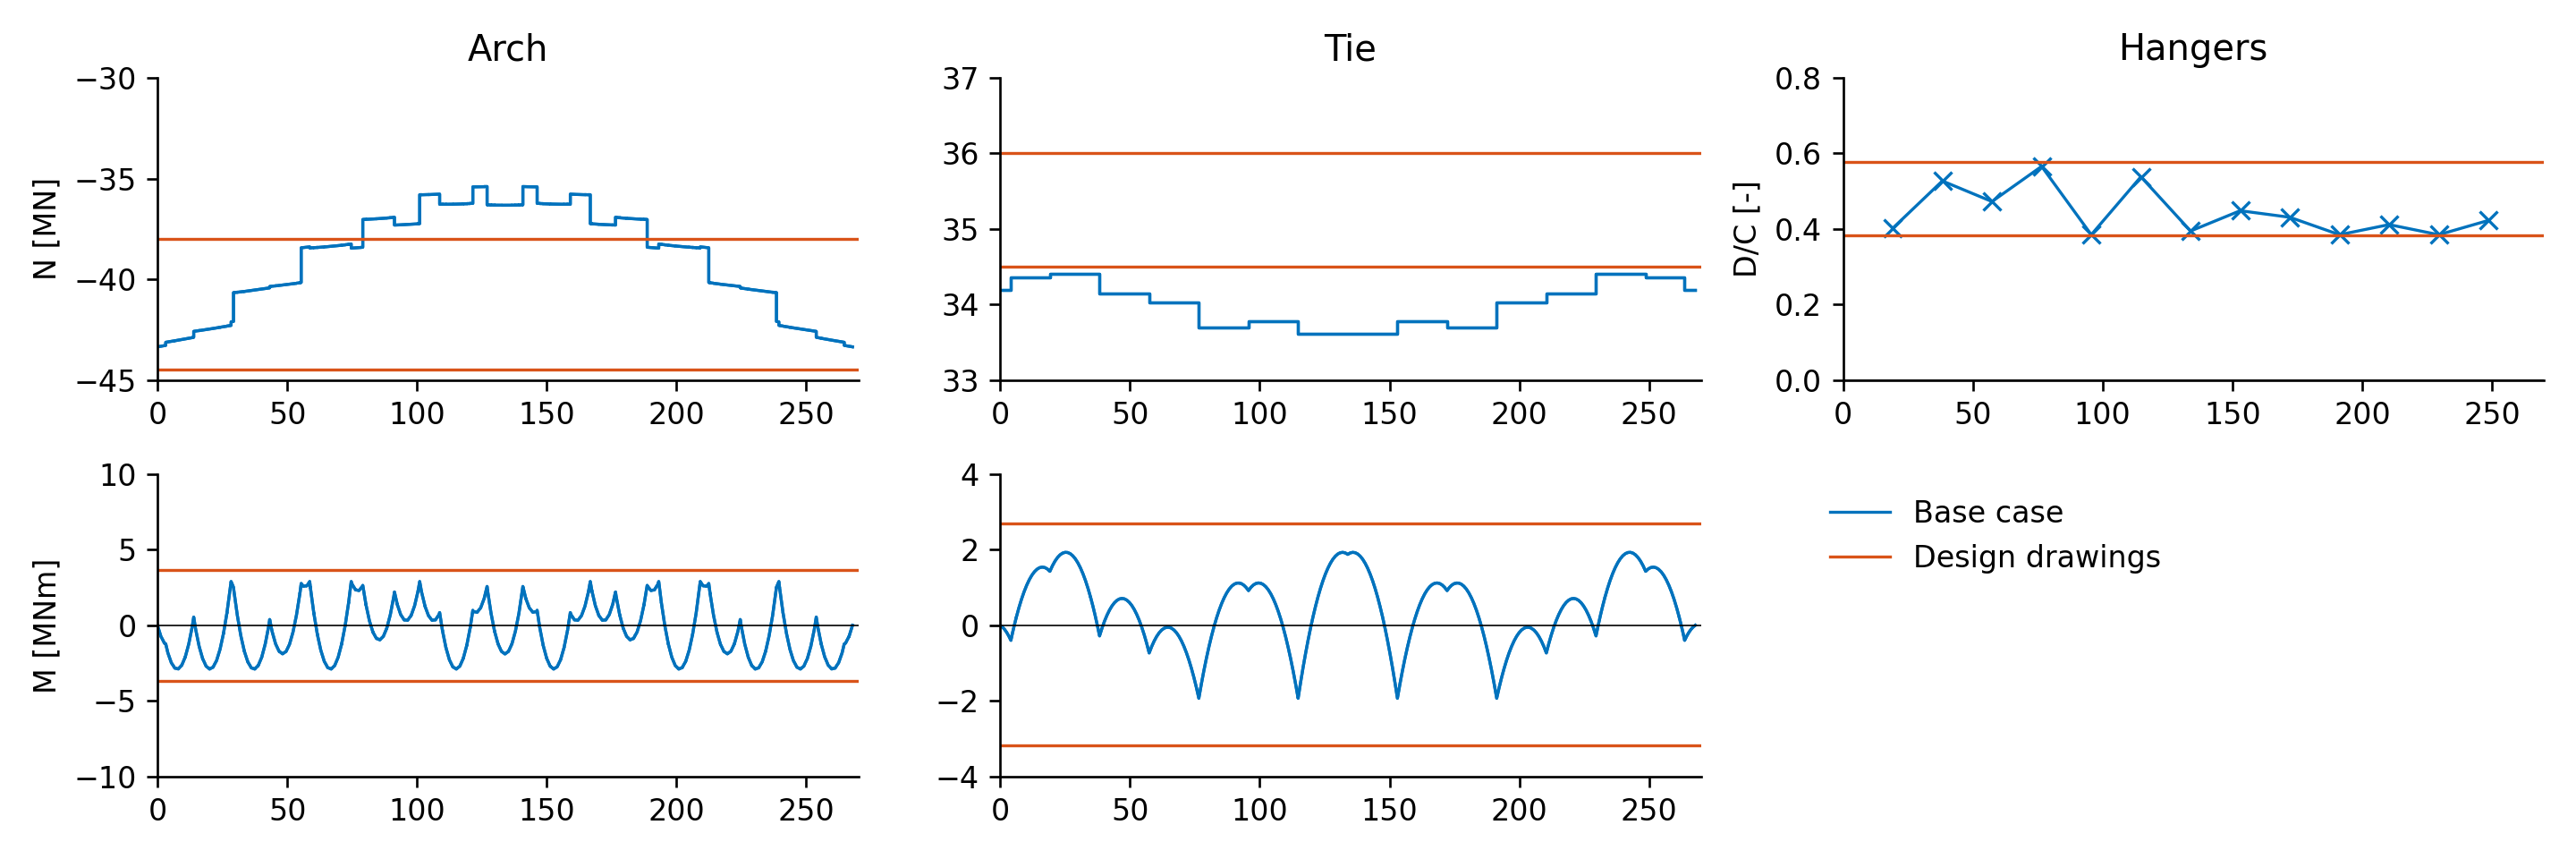
\includegraphics[width=\textwidth]{calculations/Base case/Permanent state.png}
    \caption{Permanent internal forces of the base case and reference values from the drawings}
    \label{fig:base_case_permanent}
\end{figure}

The moment distributions in the arch and the tie, as well as the normal forces in the hangers, match the design drawings very well. Only for the normal force in the arch rib and the tie girder an offset of \SI{2}{MN} can be observed. This difference is probably due to underestimating the bridge's weight and because of its simplified assignment to the beam elements. However, overall the obtained internal force distribution matches the design drawings sufficiently well. Further, it can be concluded that the simultaneous arch and tie moment optimisation yields reasonable results for a fixed arch shape. Another comparison is drawn between the effects under characteristic live loads. As there are countless live load combinations, which are to be accounted for, it makes sense to look at the entire range of possible internal forces. They are shown in \cref{fig:base_case_live} by the two blue lines representing the lower and the upper limit. These ranges are again compared to the values specified in the design verifications.

\begin{figure}[H]
    \centering
    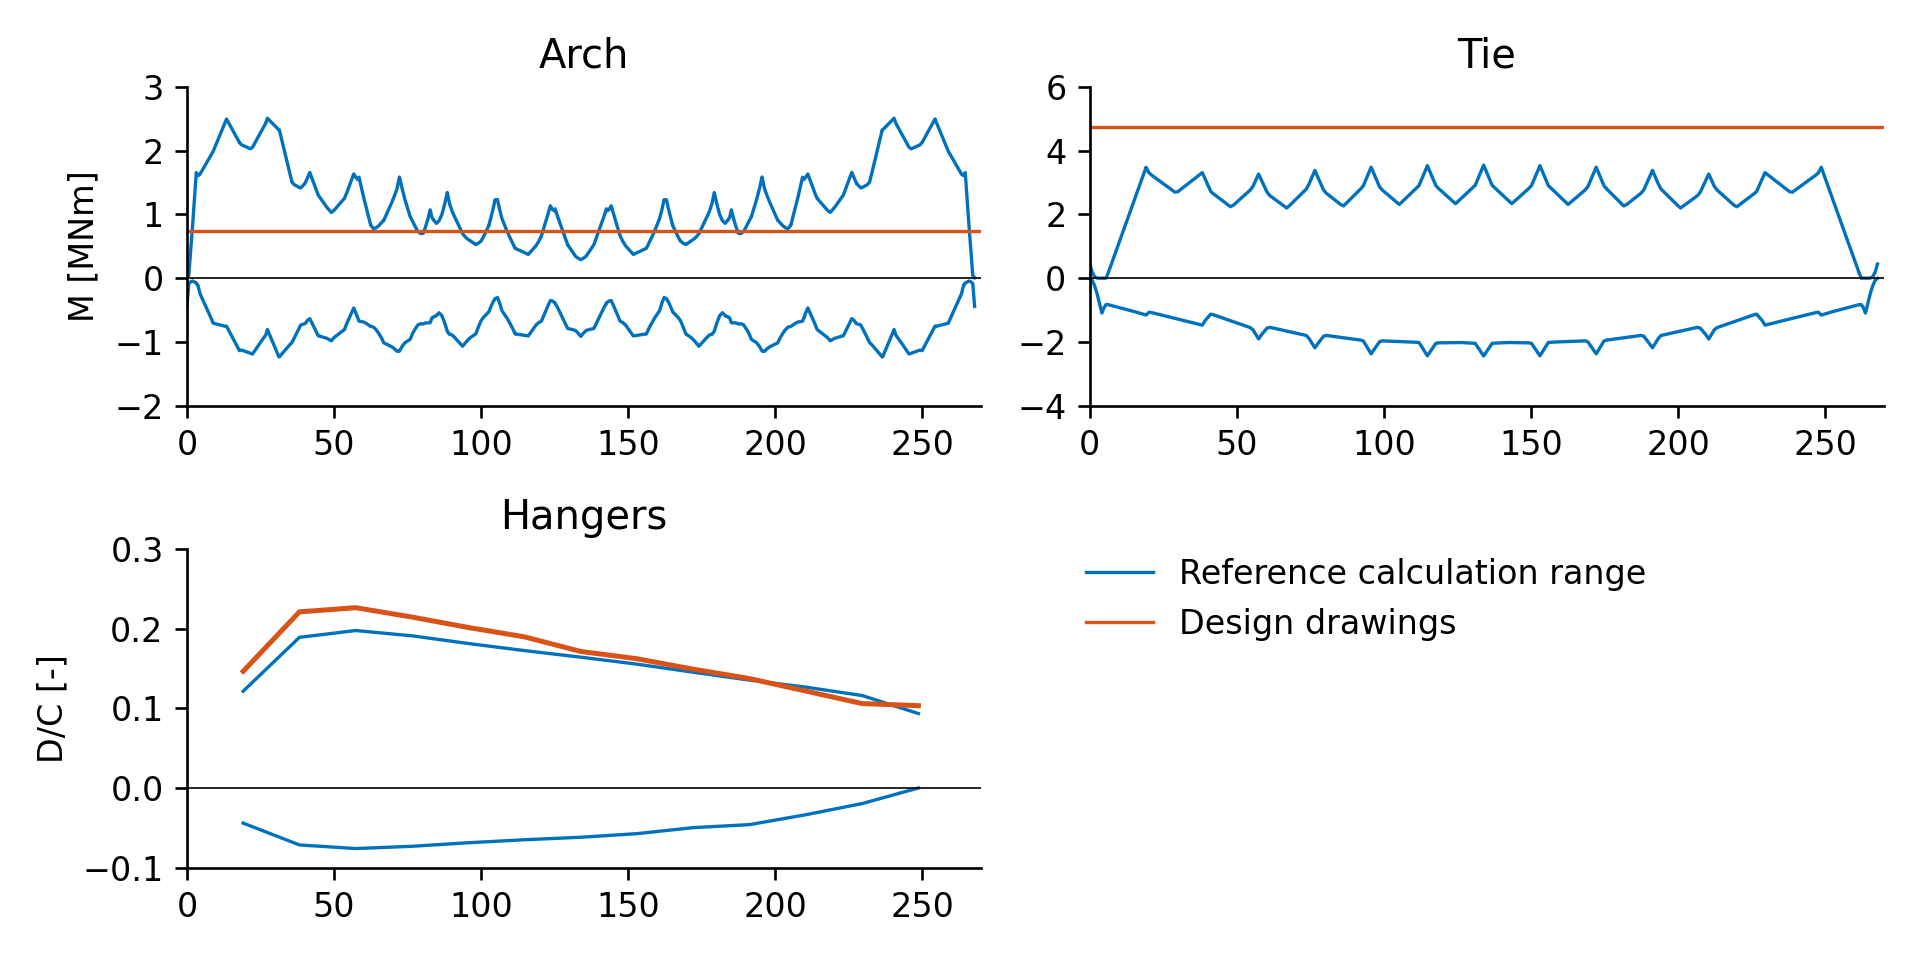
\includegraphics[width=0.8\textwidth]{calculations/Base case/Live load.png}
    \caption{Range of internal forces effects under live loading}
    \label{fig:base_case_live}
\end{figure}

The moment distribution in the arch shows a significant offset to the value given in the design drawings. However, this value cannot represent the maximum moment under live loading, considering the given hanger forces. Therefore, this difference is ignored. The moment distribution in the tie and the hangers' normal forces agree well on the other hand. The live loading is only slightly overestimated in the model, which can be seen particularly well in the hangers' demand over capacity ratios. These differences are accepted, as it is not the goal of this Thesis to reproduce the results from the design drawings. In particular, the arch segment near the knuckle is affected by strong bending moments. On the other hand, the range of effects under live loading is well distributed in the tie girder. Apparently, the influence lines for the tie girder's moments roughly follow the same shape at the different cross-girders. For the hangers, it is the second one from the knuckle connected toward the middle of the arch that undergoes the largest normal force. Towards the other side of the hanger set, the hanger forces decrease. The strongly affected hangers have in common that their inclination is closer to the arch's inclination at their respective connection node. The arch is very stiff on axial loading and comparably weaker on perpendicular forces. Therefore, at the arch nodes, smaller displacements in the hanger's direction are expected for the first hangers of the considered hanger set, explaining their higher normal forces. Only the first hanger does not follow this rule, which is explained by its smaller area of influence due to the nearby knuckle. \medskip

The resulting demand over capacity ratios for all segments and limit states are presented in Table \ref{tab:dc_base_case}. Considering the strength limit states, wind exposure is governing the segment close to the knuckle for both the arch and the tie. For the segment in the span, as well as for the hangers, it is the vehicular load that poses the highest demand. The limit state for high dead-to-live load ratios is not decisive for any segment. However, the verifications of most segments are governed by the extreme events, especially for the tie girder. The arch rib is affected by the highest demands in the event of cable loss. Despite the lower resistance for cable replacement, it never causes the highest demands. Further, it can be concluded that the estimated costs in the following investigations can only be reduced by improving the demands for the extreme events.

\begin{table}[H]
    \centering
    \caption{Demand over capacity ratios of the base case}
    \label{tab:dc_base_case}
    \input{calculations/Base case/dc table.txt}
\end{table}

A comparison to the ratios found in the design drawings, presented in Table \ref{tab:dc_drawings}, shows that the limit state for high dead-to-live load ratios can be the governing strength verification for the arch. The corresponding underestimation in the base case is probably due to a general weight underestimation, which has already been seen for the permanent effects. Nonetheless, the strength limit states agree well with the design drawings' verifications, even though slightly underestimated. On the other hand, for cable loss and replacement, the demands predicted by the considered model are overestimated. Besides the higher dynamic amplification factor of 1.75 for cable loss, this is due to the modelling of a single arch plane, which does not consider the other undamaged arch plane. Nevertheless, the results are within an acceptable range. For the tie fracture extreme event, which is considered in a simplistic manner, demands near 1.00 result. It agrees with the design drawings, in which it is only noted that the tie fracture governed the design of the tie girder. For the comparative investigations in this Thesis, the simplistic verification is adequate, as the tendencies can be modelled sufficiently accurate.

\begin{table}[H]
    \centering
    \caption{Demand over capacity ratios of the final design}
    \label{tab:dc_drawings}
    \begin{tabular}{lccccccc}
    \toprule
    Segment & \multicolumn{7}{c}{Demand / Capacity} \\
     & S-I & S-III & S-IV & Replacement & Loss & Fracture & Fatigue\\ \midrule 
    Arch 1 & - & \textbf{1.00} & - & - & 0.85 & -  & - \\ 
    Arch 2 & - & - & 0.99 & - & \textbf{1.00} & -  & - \\ 
    Arch 3 &  - & - & 0.83 & - & \textbf{0.97} & -  & - \\ 
    Tie 1 & - & 0.69 & - & - & 0.61 & $\sim$\textbf{1.00} & - \\ 
    Tie 2 & 0.68 & - & - & - & 0.88 & $\sim$\textbf{1.00} & - \\ 
    Tie 3 & 0.63 & - & - & - & 0.76 & $\sim$\textbf{1.00} & - \\ 
    Hangers & 0.91 & 0.77 & 0.75 & - & 0.74 & -  & -\\ 
    \bottomrule
\end{tabular}

\end{table}

\newpage
\section{Arch shape} \label{sec:arch_shape}
In this section, the arch shape is investigated as it affects the investigation of the following hanger-related design variables. Most network tied-arch bridges feature a parabolic arch. It is a relic of the classical tied-arch bridge with vertical hangers. 
The vertical hanger forces on the arch are evenly distributed and the respective thrust line approximately matches the parabola, if the arch weight is negligible.
For network tied-arch bridges, circular arch shapes have been considered suitable for radial arrangements. Each pair of radial hangers equals an approximately radial loading which causes a circular thrust line.
For a rise to span ratio of $r/s=0.2$, the two shapes diverge by up to 0.8\% of the span. While these differences might seem negligible on a drawing, the impact of this difference on the arch's moment distribution is significant, as it is bigger than its usual cross-section height. 
The implications are first investigated on the Blennerhassett Island Bridge in \cref{sec:arch_shape_BIB}. Afterwards, the arch shapes are studied for a denser and a continuous hanger arrangement in \cref{sec:arch_shape_increased} and \cref{sec:arch_shape_continuous}. The extreme event of cable loss is disregarded for in this investigation because its impact on the design verifications depends much more on the hanger arrangement than on the arch shape.

\subsection{Blennerhassett Island Bridge} \label{sec:arch_shape_BIB}
The typical solution to the issue of the arch shape's deviation from the thrust line is the assignment of non-uniform permanent hanger forces resulting in a thrust line similar to the arch shape. However, adapting the arch shape to the thrust line can be considered a more elegant solution. 
Multiple approaches to determine the arch shape have been introduced in Section \ref{sec:met_arch}. All of them are linked to the thrust line, which is the most efficient shape. The following four arch shapes are compared in this investigation.
\begin{enumerate}
    \item Thrust line: This shape is obtained numerically, as described in \cref{sec:discrete}, as the thrust line for the uniform hanger forces obtained from a tie moment optimisation. The respective hanger forces are equal to $N_p=\SI{1.8}{MN}$ corresponding to 28\% of their nominal resistance.
    \item Polynomial thrust line approximation: The above thrust line is approximated by a quartic function. The quartic function is obtained according to \cref{sec:polynomial_approximation} using the shape parameter $b$. The parameter is obtained by a least-squares approximation. 

    \item Spline thrust line approximation: As a second approximation of the thrust line, a cubic spline defined by the respective arch-hanger connection nodes is used. These nodes are therefore represented at their exact location. Further, the shape is characterised by a continuous curvature.
    \item Thrust line of continuous hanger arrangement: This shape is the thrust line of the hypothetical continuous hanger arrangement, which was introduced in \cref{sec:continuous}.
\end{enumerate}

Instead of the arch shapes, the respective deviations to the parabola are shown in \cref{fig:arch_shapes_13} to make their differences visible. 
Also, a circular arch is shown to put the results into perspective.

\begin{figure}[H]
    \centering
    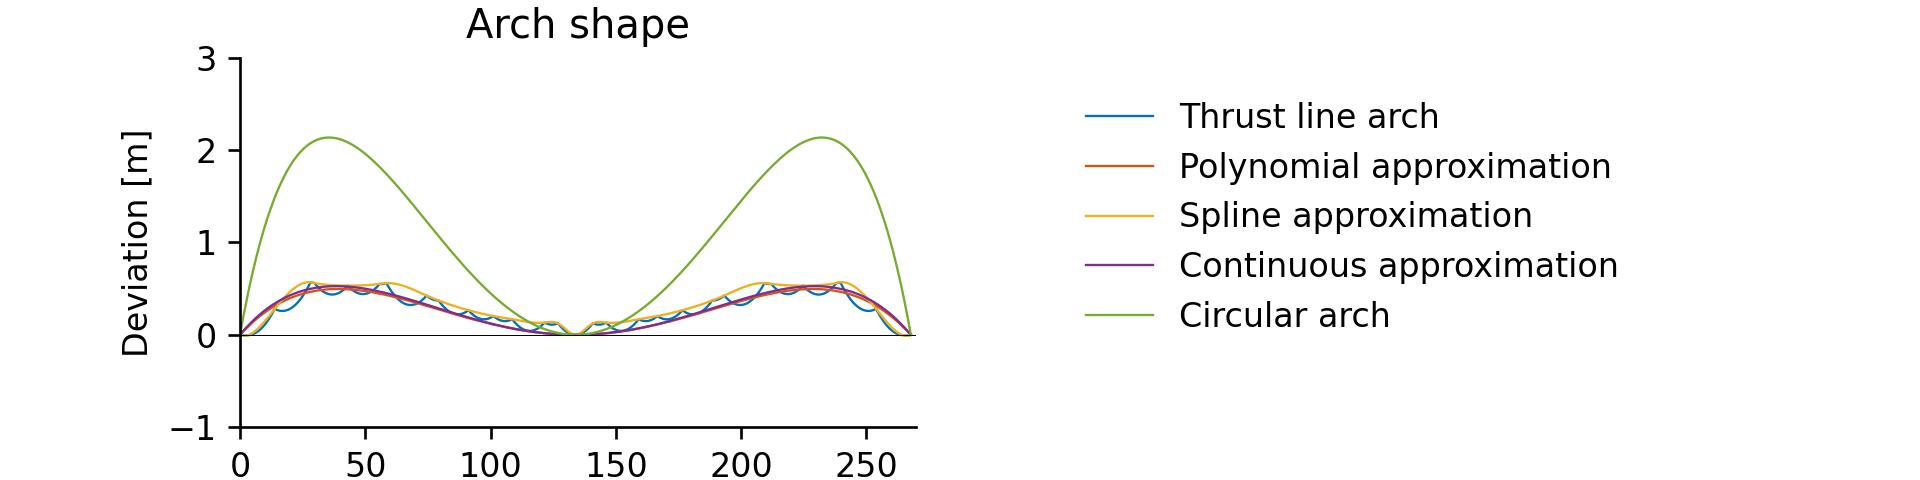
\includegraphics[trim={1cm 0 3cm 0.45cm},clip, width=0.79\textwidth]{calculations/arch shape/arch_shapes_13.png}
    \caption{Deviation of arch shapes to the parabola}
    \label{fig:arch_shapes_13}
\end{figure}

The thrust line tends slightly to the parabolic side in the range between the circular and the parabolic shape. All three approximations seem to fit the thrust line reasonably well. However, to investigate the impacts of the remaining deviations from the thrust line, the corresponding permanent moment distribution is presented in \cref{fig:arch_permanent_moments_13}. Further, from the similarity between the polynomial and the continuous approximation, it can be concluded that a quartic function can yield an appropriate arch shape for this hanger arrangement. 

\begin{figure}[H]
    \centering
    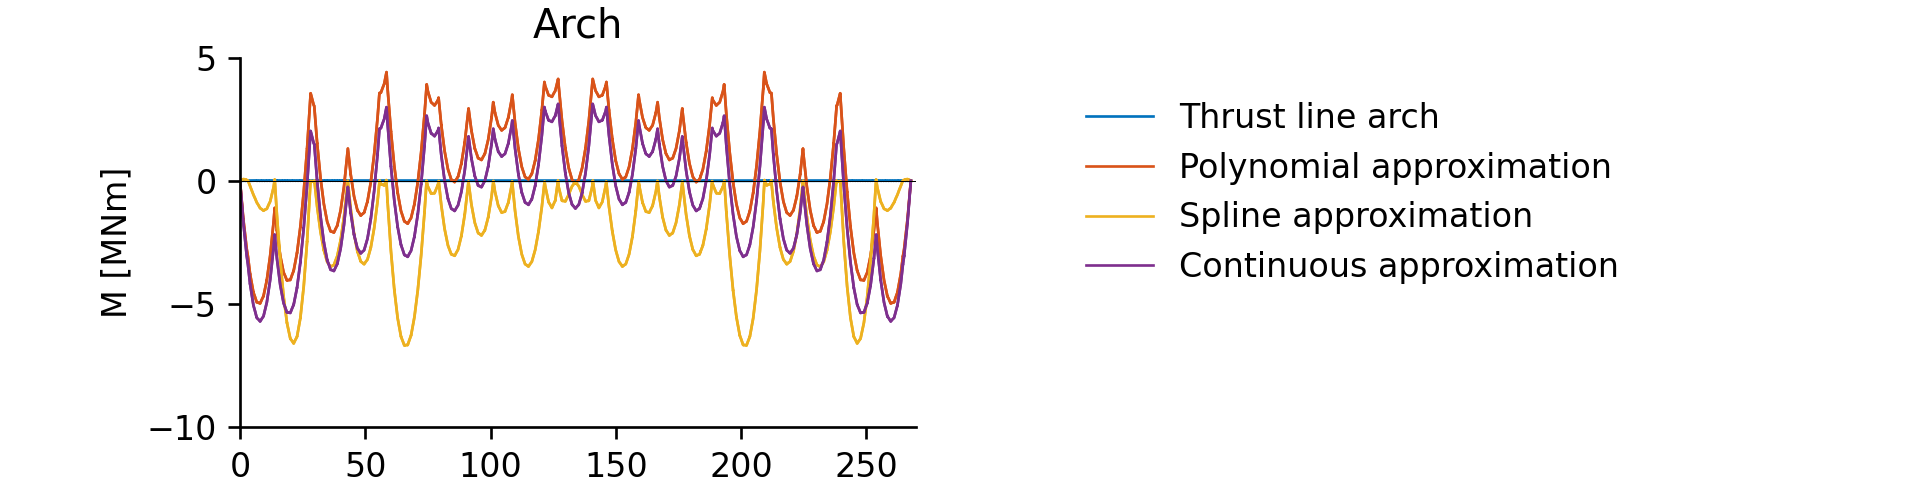
\includegraphics[trim={1cm 0 3cm 0.48cm},clip, width=0.76\textwidth]{calculations/arch shape/permanent state_13.png}
    \caption{Permanent arch moment distributions depending on arch shape}
    \label{fig:arch_permanent_moments_13}
\end{figure}

Despite the apparent match of the arch shapes, significant bending moments result in each of the three approximations. Interestingly, all approximations feature a similar parabolic moment distribution between the arch-hanger connection nodes. The spline approximation's moment distribution is strictly negative, which relies on the characteristic that a spline lies above the approximately linear thrust line and only matches it at the connection nodes. While these moment distributions resulting for the approximated shapes are certainly considerable, it is infeasible to find a continuously curved shape matching the arch thrust line. Any shape with an approximately constant radius $R$ between two nodes results in a deviation from the approximately linear thrust line and causes the corresponding deviation moment $\Delta M$. This deviation can be approximated depending on the distance between two hanger connection nodes $d$ and the arch's normal force $N$ according to \cref{eq:moment_deviation}.

\begin{equation}
    \Delta M=-\left(R-\sqrt{R^2-\left(d/2\right)^2}\right) \cdot N
    \label{eq:moment_deviation}
\end{equation}

For the Blennerhassett Island Bridge, these variables roughly correspond to $R=\SI{194}{m}$, $d=\SI{17}{m}$ and $N=\SI{40}{MN}$. \cref{eq:moment_deviation} yields a deviation moment of $\Delta M=\SI{7.5}{MNm}$ providing a good match for the value observed in \cref{fig:arch_permanent_moments_13}. From the analytical form of \cref{eq:moment_deviation} it can further be concluded that a reduction of the hanger node spacing has a more than proportional impact on the deviation moment. From this perspective, an optimum hanger arrangement features one hanger per connection node and a uniform spacing on the arch. Considering the number of hangers and the arch's length, a minimum spacing of $d=\SI{11}{m}$ can be obtained. Thereby, the deviation moment reduces to $\Delta M=\SI{3.1}{MNm}$ corresponding to a reduction of the D/C ratio of 0.03.
To also put the deviations of the approximated shapes into the context of the design verifications, the demand over capacity ratios resulting in the arch are shown in Table \ref{tab:arch_shape_dc_13} along with the decisive limit state.

\begin{table}[H]
    \centering
    \caption{Arch design verifications for different arch shapes}
    \label{tab:arch_shape_dc_13}
    \input{calculations/arch shape/dc_comparison_13.txt}
\end{table}

The deviations from the thrust line of the considered arch shapes increase the D/C ratios by 0.06 on average. This difference is not critical for the initial design, but it offers some potential for optimisation. Further, it should be noted that also, the exact thrust line is not the most efficient arch shape. In the strength limit state for vehicular use, the arch is affected by stronger positive bending moments than negative ones, as shown in \cref{fig:arch_shape_strength_1} for the arch shape corresponding to the thrust line. Therefore, a certain upward deviation from the thrust line and the resulting negative bending moment can prove beneficial to the verifications. This potential was estimated by evaluating the difference between the maximum and minimum bending moments in the decisive limit state and comparing it to the resistance. The comparison yielded possible reductions of the D/C ratio between 0.01 and 0.03 for the three segments.

\begin{figure}[H]
    \centering
    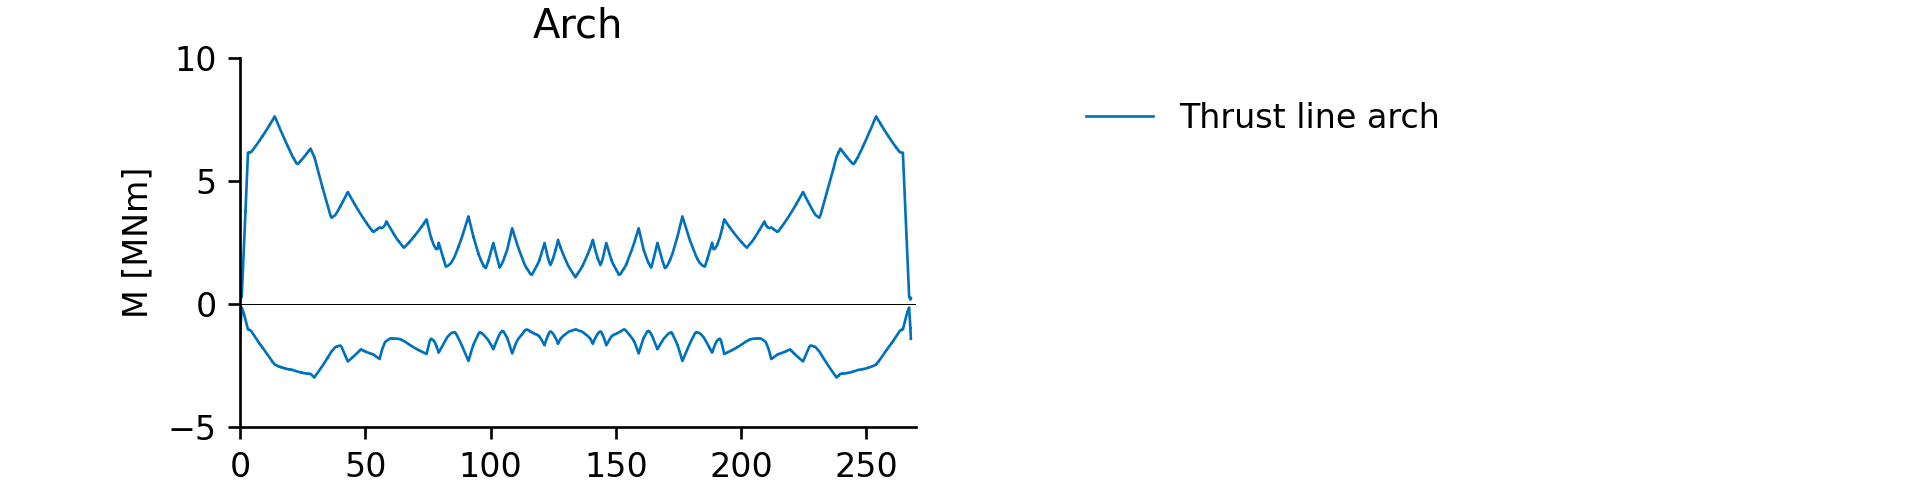
\includegraphics[trim={1cm 0 10cm 0.48cm},clip, width=0.45\textwidth]{calculations/arch shape/strength-I_13.png}
    \caption{Range of moments in the Strength-I limit state for a thrust line arch shape}
    \label{fig:arch_shape_strength_1}
\end{figure}

\subsection{Increased hanger density} \label{sec:arch_shape_increased}
In this section, the influence of the hanger density on the arch shape is investigated. It was concluded from \cref{eq:moment_deviation} that reducing the distances between the hangers an over-proportional reduction in the permanent moment distribution results. Therefore, a similar calculation of the four arch shapes with 26 hangers per set is conducted. The resulting arch shapes are presented in \cref{fig:arch_shapes_26}.

\begin{figure}[H]
    \centering
    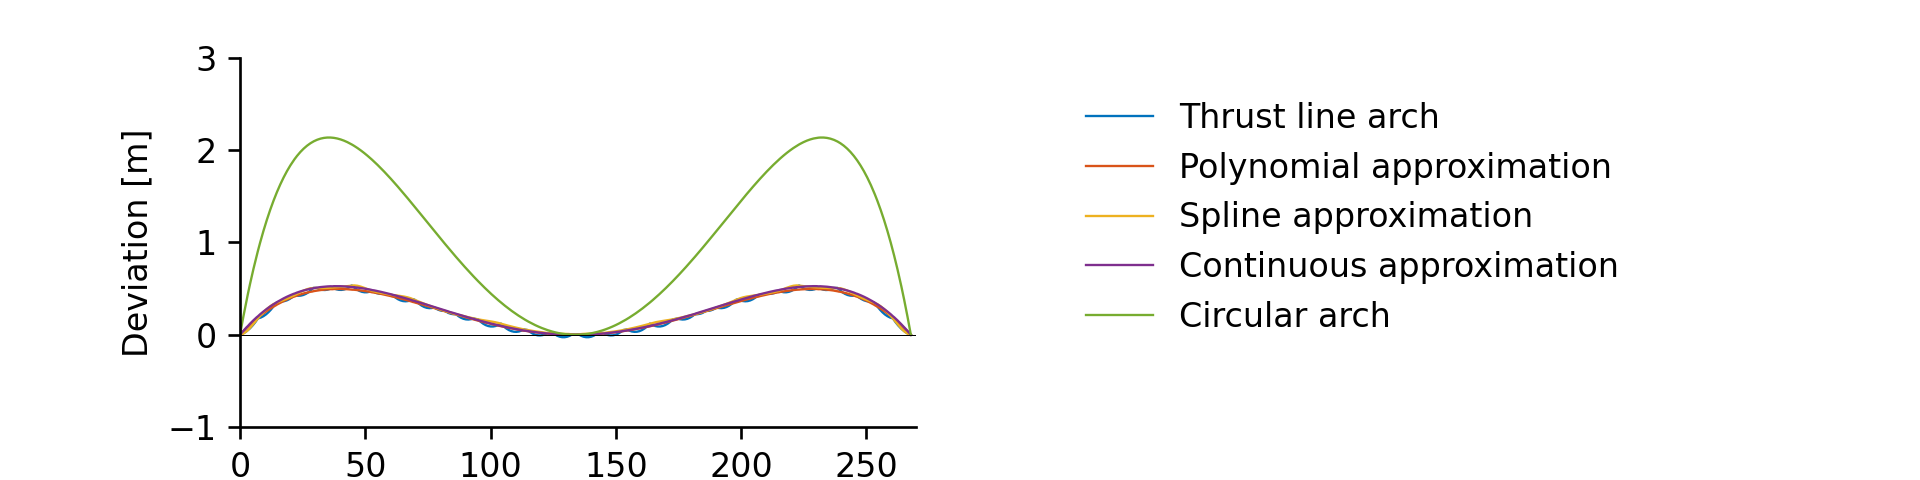
\includegraphics[trim={1cm 0 3cm 0.48cm},clip, width=0.7\textwidth]{calculations/arch shape/arch_shapes_26.png}
    \caption{Deviation of arch shapes from parabolic shape (26 hangers)}
    \label{fig:arch_shapes_26}
\end{figure}

If the amount of hangers is large enough, all considered approximations yield suitable arch shapes. The impact of the remaining deviation from the thrust line on the design verifications is negligible, as shown in the uniform demand over capacity ratios presented in Table \ref{tab:arch_shape_dc_26}.

\begin{table}[H]
    \centering
    \caption{Arch design verifications (26 hangers)}
    \label{tab:arch_shape_dc_26}
    \input{calculations/arch shape/dc_comparison_26.txt}
\end{table}

\subsection{Continuous hanger arrangement} \label{sec:arch_shape_continuous}
For the initial design, the continuous approximation presents a promising arch shape, as it does not involve a specific thrust line calculation and has a continuous radius of curvature. In this section, the respective shape of a selection of hanger arrangements is presented. The investigated arrangements are three parallel arrangement with inclinations of $45\degree$, $65\degree$ and $85\degree$. Also, an arrangement with a constant change of inclination from $85\degree$ to $45\degree$ and two radial arrangements with intersection angles of $20\degree$ and $35\degree$ are investigated. The respective continuous thrust lines are shown in \cref{fig:continuous_thrust_lines}.

\begin{figure}[H]
    \centering
    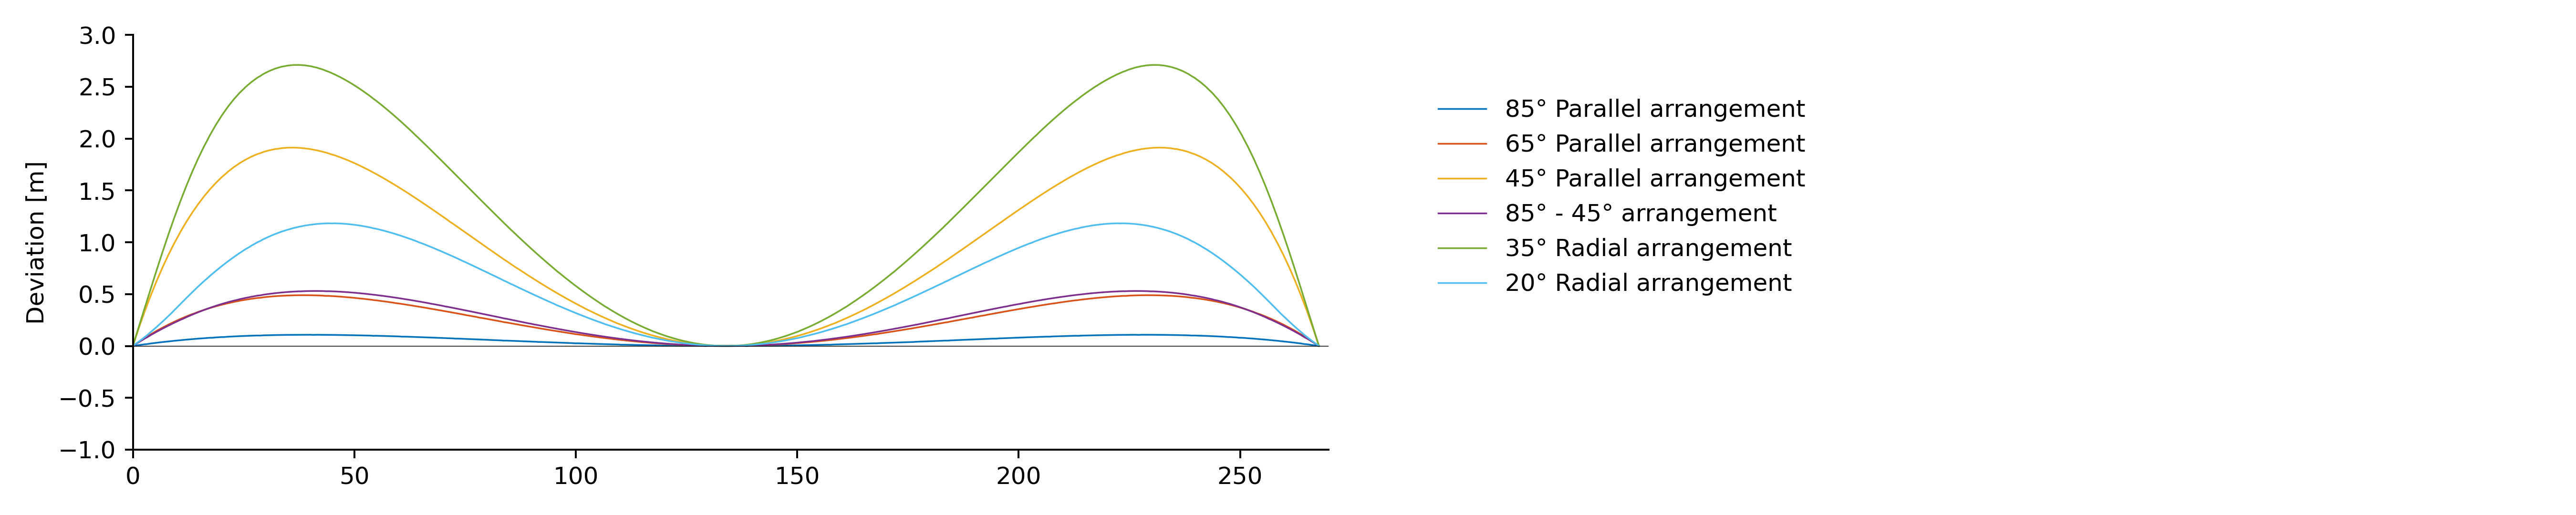
\includegraphics[trim={0 0 55cm 0},clip, width=0.9\textwidth]{overleaf/Pictures/myplot_3.png}
    \caption{Deviation of the continuous thrust lines from parabolic shape}
    \label{fig:continuous_thrust_lines}
\end{figure}

The 85\degree parallel arrangement's thrust line almost corresponds to the parabolic shape, which was expected from the classical network arch bridges. The $65\degree$ arrangement lies between the circle and the parabola similar to the case of the Blennerhassett Island Bridge. Interestingly, the constant change of inclination arrangement with an average angle of $65\degree$ has an almost identical thrust line. Surprisingly, not the radial arrangements but the $45\degree$ arrangement has a circular thrust line. This is due to the perpendicular hangers, which are affected by a uniform permanent hanger force density. This forms a biaxial stress state within the network arch and explains the circular thrust line. The radial arrangements show a clear offset to the circle. The $\beta=35\degree$ arrangement even lies outside of the range between the circle and the parabola. It can be expected that with a parameter of $\beta=28\degree$ the circle provides a good fit. However, for general radial arrangements, a more elaborate consideration seems appropriate. In the next step, it is checked whether a quartic polynomial can approximate these shapes. The parameter $b$, which was introduced in \cref{sec:polynomial_approximation}, is fitted by a least-squares analysis to the continuous thrust lines. The obtained values are shown in \cref{tab:approximate} along with the maximum difference between the thrust line and the approximation.

\begin{table}[H]
    \caption{Polynomial approximation of the continuous thrust lines}
    \label{tab:approximate}
    \begin{subtable}{.5\linewidth}
        \centering
        \caption{Parameter $b$}
        \label{tab:approximate_b}
        \resizebox{!}{1.8cm}{%
        \begin{tabular}{lcccccccc}
\toprule
\multicolumn{9}{l}{\bf{Constant change of inclination arrangement}} \\
$\alpha_1$ &  & 105\degree & 95\degree & 85\degree & 75\degree & 65\degree & 55\degree & 45\degree \\ \midrule
\multirow{5}{*}{$\alpha_{mid}$} & 85\degree & 0.984 & 0.990 & 0.992 & - & - & - & - \\
 & 75\degree & 0.968 & 0.977 & 0.982 & 0.983 & - & - & - \\
 & 65\degree & 0.943 & 0.953 & 0.960 & 0.964 & 0.964 & - & - \\
 & 55\degree & 0.910 & 0.921 & 0.929 & 0.932 & 0.932 & 0.927 & - \\
 & 45\degree & - & - & 0.891 & 0.891 & 0.885 & 0.875 & 0.859 \\ \midrule
\multicolumn{9}{l}{\bf{Radial arrangement}} \\
$\beta$ & 0\degree & 5\degree & 15\degree & 20\degree & 25\degree & 30\degree & 35\degree & 40\degree \\ \midrule
b & 0.945 & 0.940 & 0.929 & 0.914 & 0.890 & 0.855 & 0.802 & 0.712  \\ \bottomrule
\end{tabular}
        }    
    \end{subtable}%
    \begin{subtable}{.5\linewidth}
        \centering
        \caption{Maximum difference $\Delta_{max}$}
        \label{tab:approximate_dif}
        \resizebox{!}{1.8cm}{%
        \begin{tabular}{lccccccccl}
\toprule
\multicolumn{9}{l}{\bf{Constant change of inclination arrangement}} & \\
$\alpha_1$ &  & 105\degree & 95\degree & 85\degree & 75\degree & 65\degree & 55\degree & 45\degree & \\ \midrule
\multirow{5}{*}{$\alpha_{mid}$} & 85\degree & 0.040 & 0.012 & 0.001 & - & - & - & - & [m] \\
 & 75\degree & 0.073 & 0.036 & 0.009 & 0.001 & - & - & - & [m] \\
 & 65\degree & 0.093 & 0.058 & 0.025 & 0.001 & 0.007 & - & - & [m] \\
 & 55\degree & 0.066 & 0.049 & 0.019 & 0.013 & 0.028 & 0.031 & - & [m] \\
 & 45\degree & - & - & 0.059 & 0.081 & 0.106 & 0.121 & 0.124 & [m] \\ \midrule
\multicolumn{9}{l}{\bf{Radial arrangement}} \\
$\beta$ & 0\degree & 5\degree & 15\degree & 20\degree & 25\degree & 30\degree & 35\degree & 40\degree & \\ \midrule
$\Delta_{max}$ & 0.207 & 0.207 & 0.204 & 0.197 & 0.179 & 0.134 & 0.106 & 0.539 & [m] \\ \bottomrule
\end{tabular}
        }
    \end{subtable} 
\end{table}

For the parallel and the constant change of inclination arrangement, the polynomial approximation fits the typical inclinations from $85\degree$ to $55\degree$ for $\alpha$ or $\alpha_1$ and $\alpha_{mid}$ respectively. The corresponding deviations lie below \SI{3}{cm}. However, the quartic polynomial is not suitable for the radial arrangement with deviations higher than \SI{10}{cm}.

\newpage
\section{Hanger density} \label{sec:hanger_density}
A denser hanger arrangement provides multiple benefits. As seen in the previous chapter, the shape deviation moments are minimised by reducing the distances between the hangers' anchorages on the arch. Further, the effects in the extreme event of cable loss are significantly lowered, as the hanger forces are reduced with the increase of hangers. 
%Also, the impaired structural system also loses less of its essential stiffness and undergoes additional lower effects. 
However, the challenging task is to find an appropriate self-equilibrium stress state for structural systems in which the locations of the floor beams and the hangers do not coincide on the tie girder. 
In this investigation, this task is addressed using the tie moment optimisation method. It allows finding the permanent hanger forces minimising the resulting moment distribution in the tie girder. The hanger forces are limited between 25\% and 40\% of the hangers' characteristic capacity. First, the optimisation potential is investigated for the parallel hanger arrangement in \cref{sec:density_parallel}. Further, the optimisation potential for a dense radial arrangement is considered in \cref{sec:density_radial}.

\subsection{Parallel arrangement} \label{sec:density_parallel}
Four bridges are analysed featuring 13, 20, 26 or 27 hangers per set and a constant number of 13 floor beams. The arch shapes are defined as the quartic polynomial approximation of the thrust line. The model featuring 26 hangers is shown in \cref{fig:structure_26}. The spacing between the knuckle and the first hanger is slightly increased, so there is an equally spaced pair of hangers around every floor beam. While the arrangement appears dense, the hanger spacing on the tie girder is still around \SI{10}{m} representing a high value compared to the other network tied-arch bridges.

\begin{figure}[H]
    \centering
    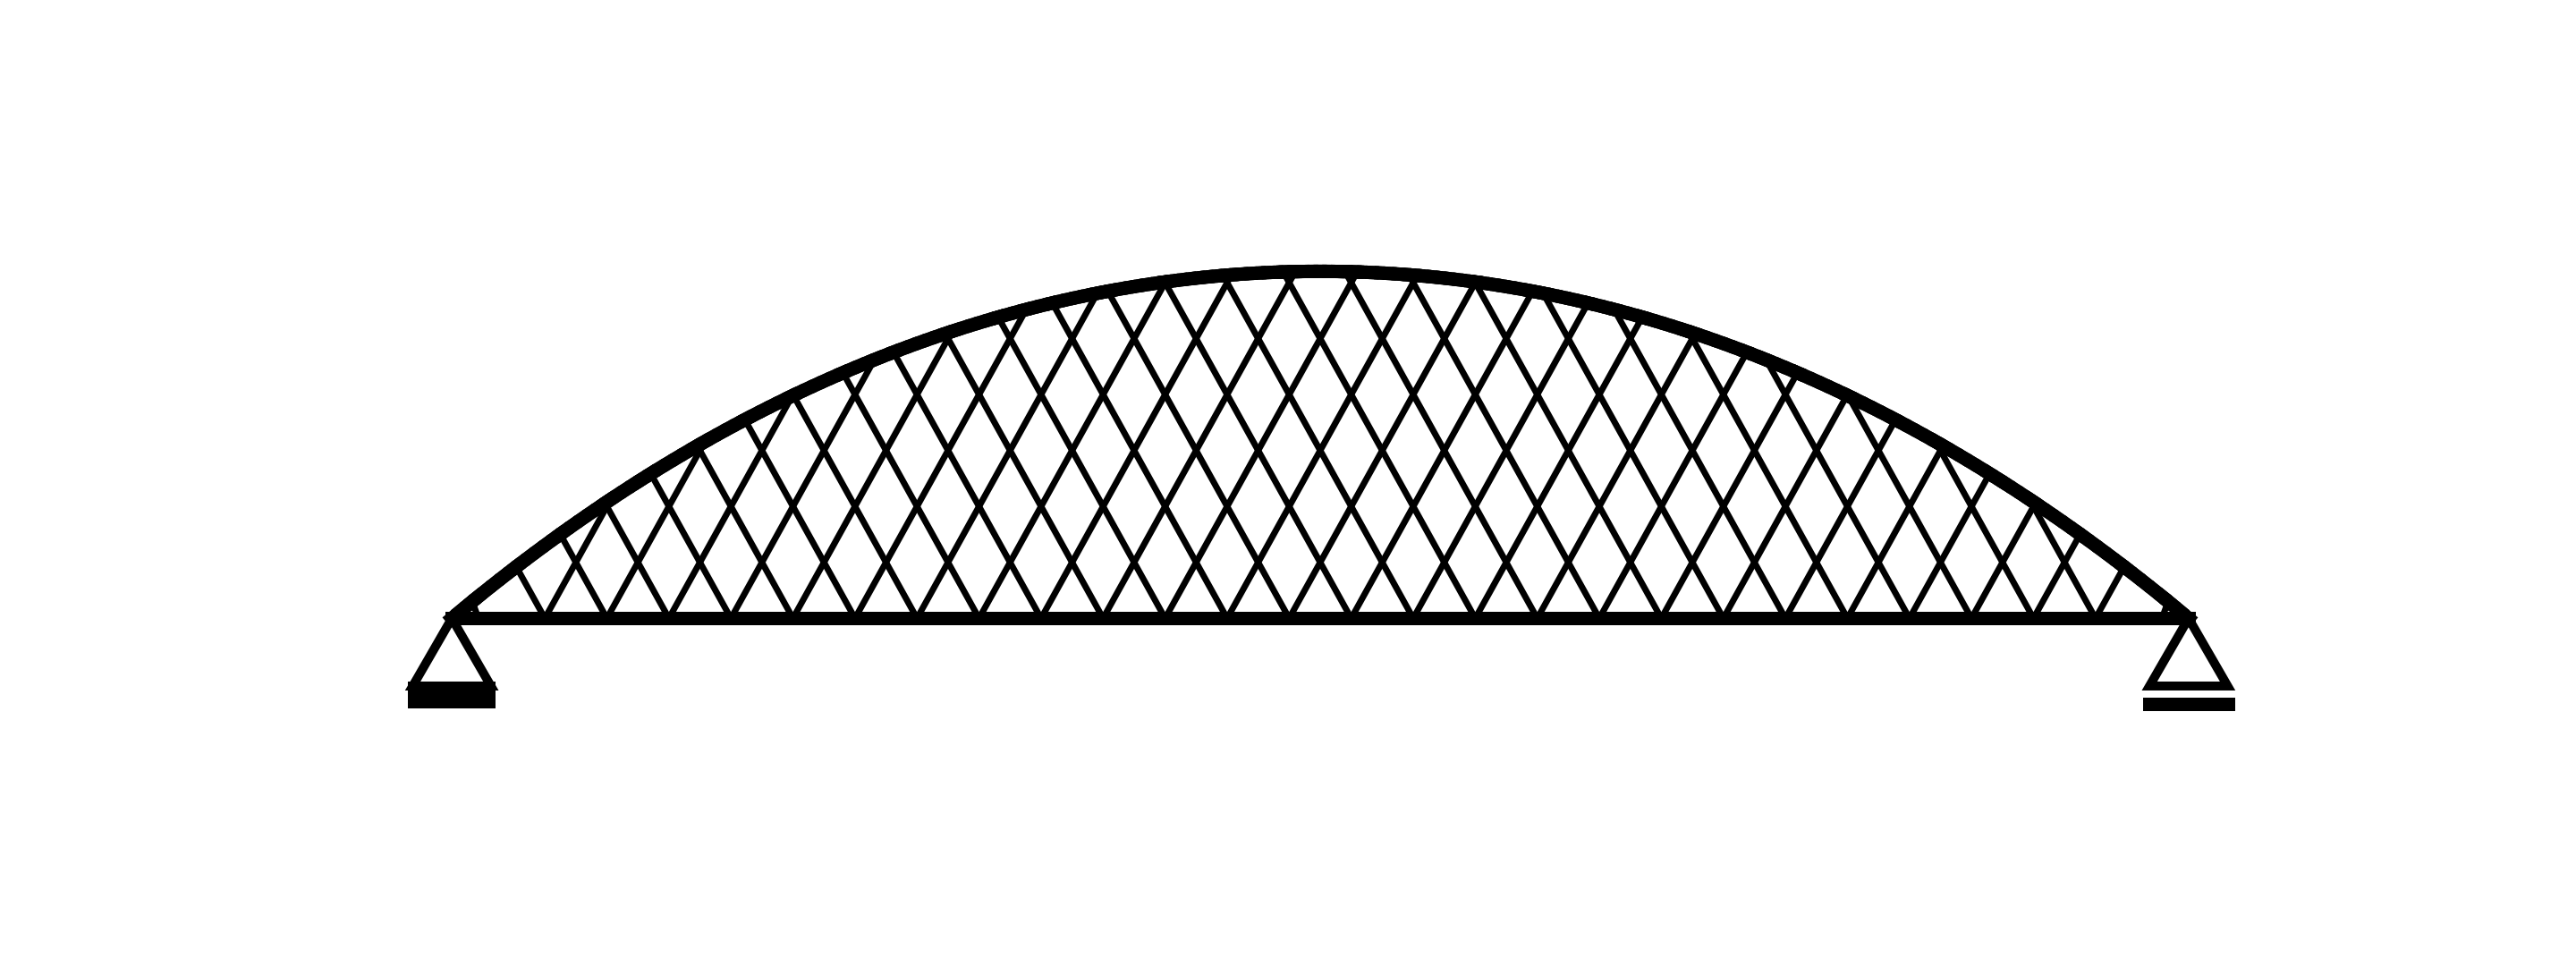
\includegraphics[trim={0 1cm 0 1cm},clip, width=0.65\textwidth]{calculations/hanger density/structure_26.png}
    \caption{Structural model of a dense hanger arrangement with 26 hangers per set}
    \label{fig:structure_26}
\end{figure}

The optimised effects under permanent loads are shown in Fig \ref{fig:hd_permanent}. As predicted by the arch shape's investigation, the bending moments in the arch are lowered for an increased hanger density. However, in the knuckle region of the arch, the significant bending moments are retained for the dense arrangements. They are due to the tie moment optimisation method assigning significant supernumerary moments to the knuckle. The quartic polynomial approximation is not able to match the corresponding thrust line. Further, the permanent hanger forces are no longer constant for the models with 20 and 27 hangers, as the hangers near the floor beams carry the majority of the forces. At the same time, a strong bending moment distribution in the tie is inevitable. The model featuring 26 hangers seems slightly more suitable as it can retain constant hanger forces and a slightly lower tie moment distribution.

\begin{figure}[H]
    \centering
    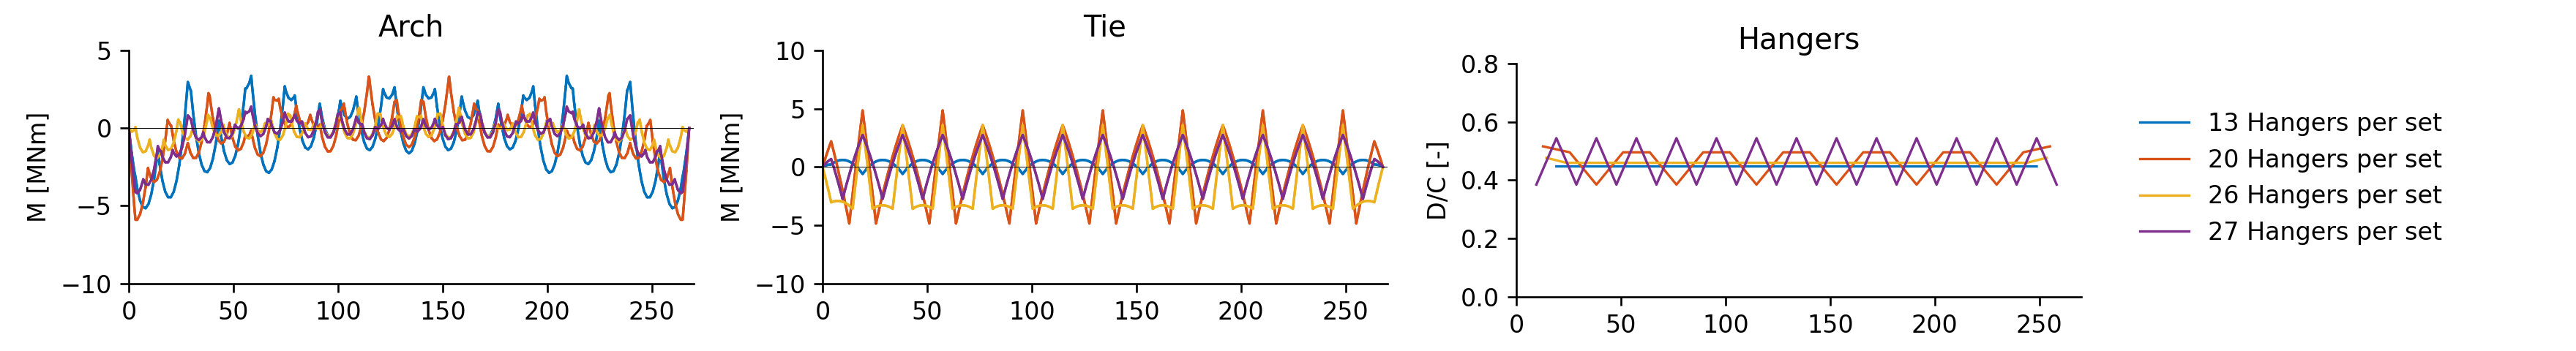
\includegraphics[trim={0 0 2cm 0},clip, width=\textwidth]{calculations/hanger density/permanent_plot.png}
    \caption{Optimised permanent effects for different hanger densities}
    \label{fig:hd_permanent}
\end{figure}

The elastic responses to dead loading are shown in \cref{fig:hd_elastic_response_dl}.
%On top of the disadvantageous permanent effects, the modified models' elastic response to live loading, shown in \cref{fig:hd_live}, seems unfavourable.

\begin{figure}[H]
    \centering
    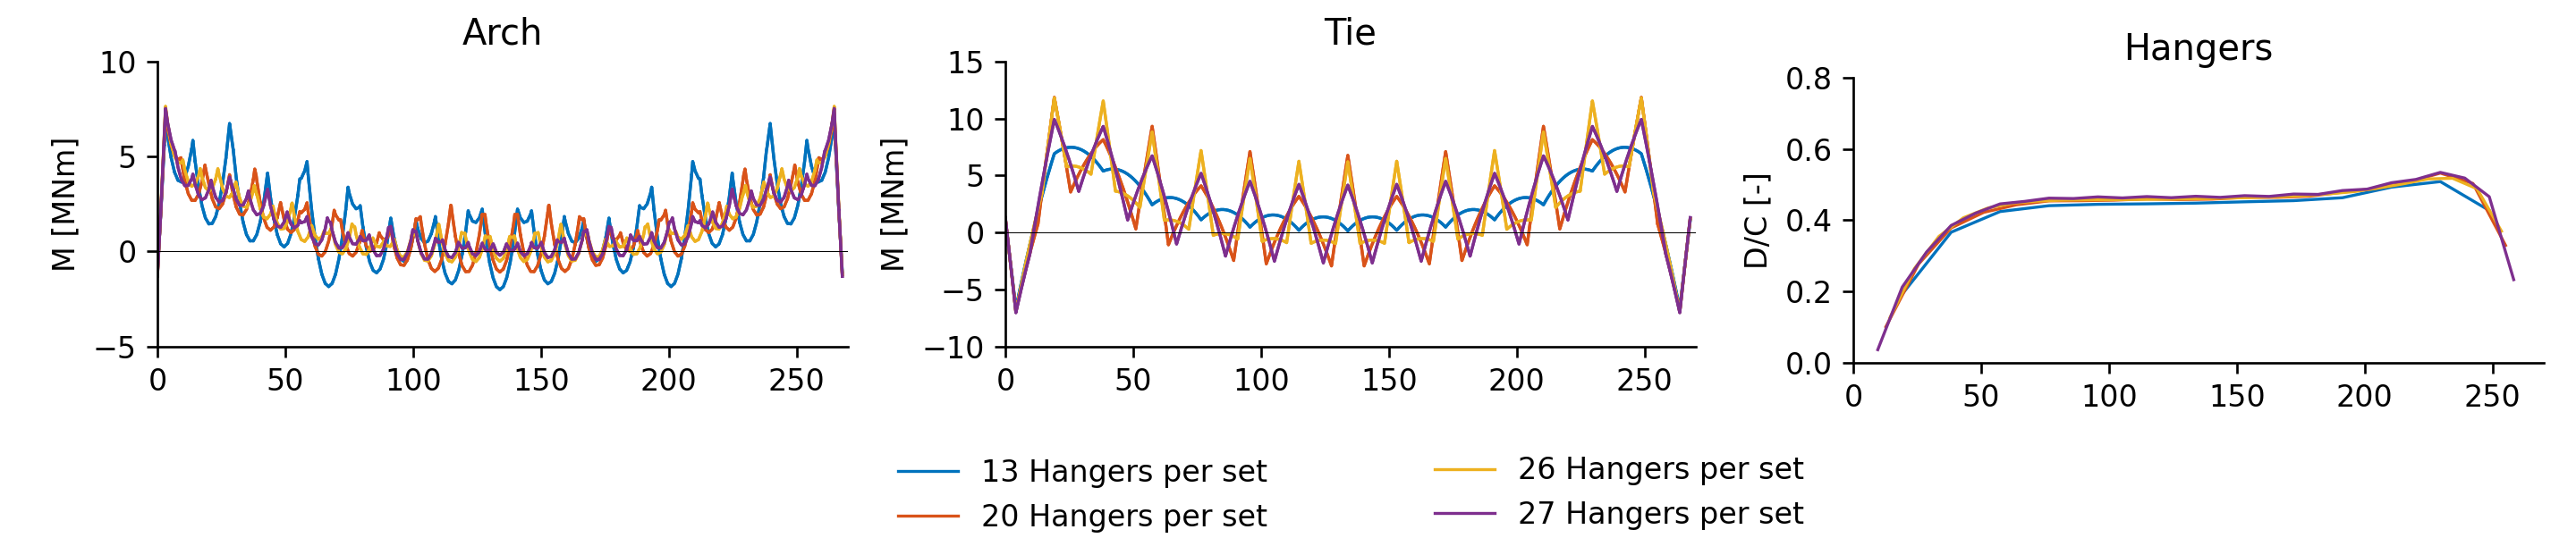
\includegraphics[trim={0 0 1cm 0},clip, width=\textwidth]{calculations/hanger density/dead loading_plot.png}
    \caption{Elastic response to dead loading for different hanger densities}
    \label{fig:hd_elastic_response_dl}
\end{figure}

While the effects for characteristic dead loads are already included in the permanent effects, they are still relevant for the design verifications as they are increased or decreased depending on the limit state. For the arch, the increased number of hangers reduced the moment distribution peaks similar to the permanent state. Also, the hangers show similar effects. Only the ones close to the knuckle are seen to carry little of the dead loading. This issue is addressed in the investigation of the hanger inclination in \cref{sec:inclination}.
The tie girder is again affected by stronger bending moments in the denser models. This characteristic is accentuated by the range of tie moments relevant for the tie fracture extreme event, presented in \cref{fig:hd_tie_fracture}.

\begin{figure}[H]
    \centering
    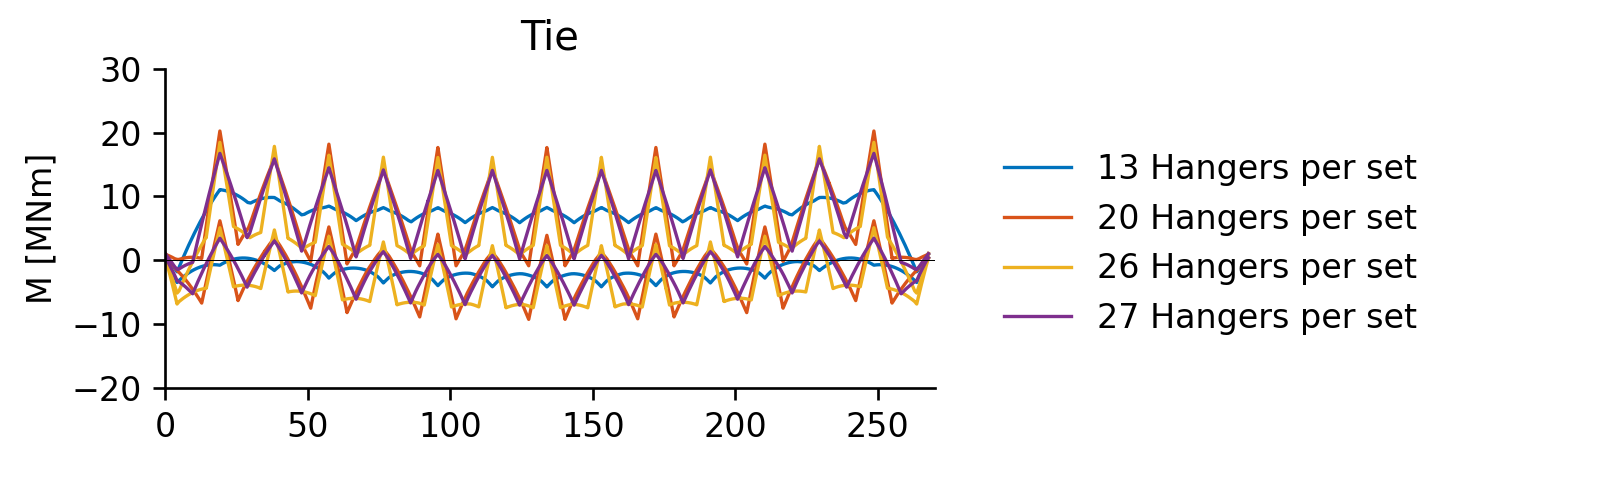
\includegraphics[trim={0 0 3cm 0},clip, width=0.7\textwidth]{calculations/hanger density/tie fracture_plot.png}
    \caption{Range of tie bending moment for tie fracture extreme event}
    \label{fig:hd_tie_fracture}
\end{figure}

The uniform moments from the final design become particularly peaky if more hangers are arranged. The corresponding design verification in the tie is thereby significantly impaired, as shown in \cref{tab:hd_dc}. An optimisation of the hanger density itself, therefore renders no potential for optimisation, even though the cable loss extreme event improves as expected.

\begin{table}[H]
    \centering
    \caption{Design verifications for different hanger densities}
    \label{tab:hd_dc}
    \resizebox{\columnwidth}{!}{%
    \input{calculations/hanger density/dc_comparison.txt}
    }
\end{table}

\subsection{Radial arrangement} \label{sec:density_radial}
In many investigations, the radial arrangement has been considered the most advantageous. However, it is an even more challenging task to find a suitable self-equilibrium stress state as the spacing on the tie girder varies strongly. In this section, it is investigated whether it is possible to obtain state allowing for its further consideration. Therefore, three radial hanger arrangements featuring 13, 20 and 26 hangers per set and characteristic angle of $\beta=\SI{25}{\degree}$ are investigated. 
As the polynomial approximation does not yield a sufficient approximation, the spline approximation is considered for these models. The structural model for the densest arrangement is shown in \cref{fig:structure_26_radial}.

\begin{figure}[H]
    \centering
    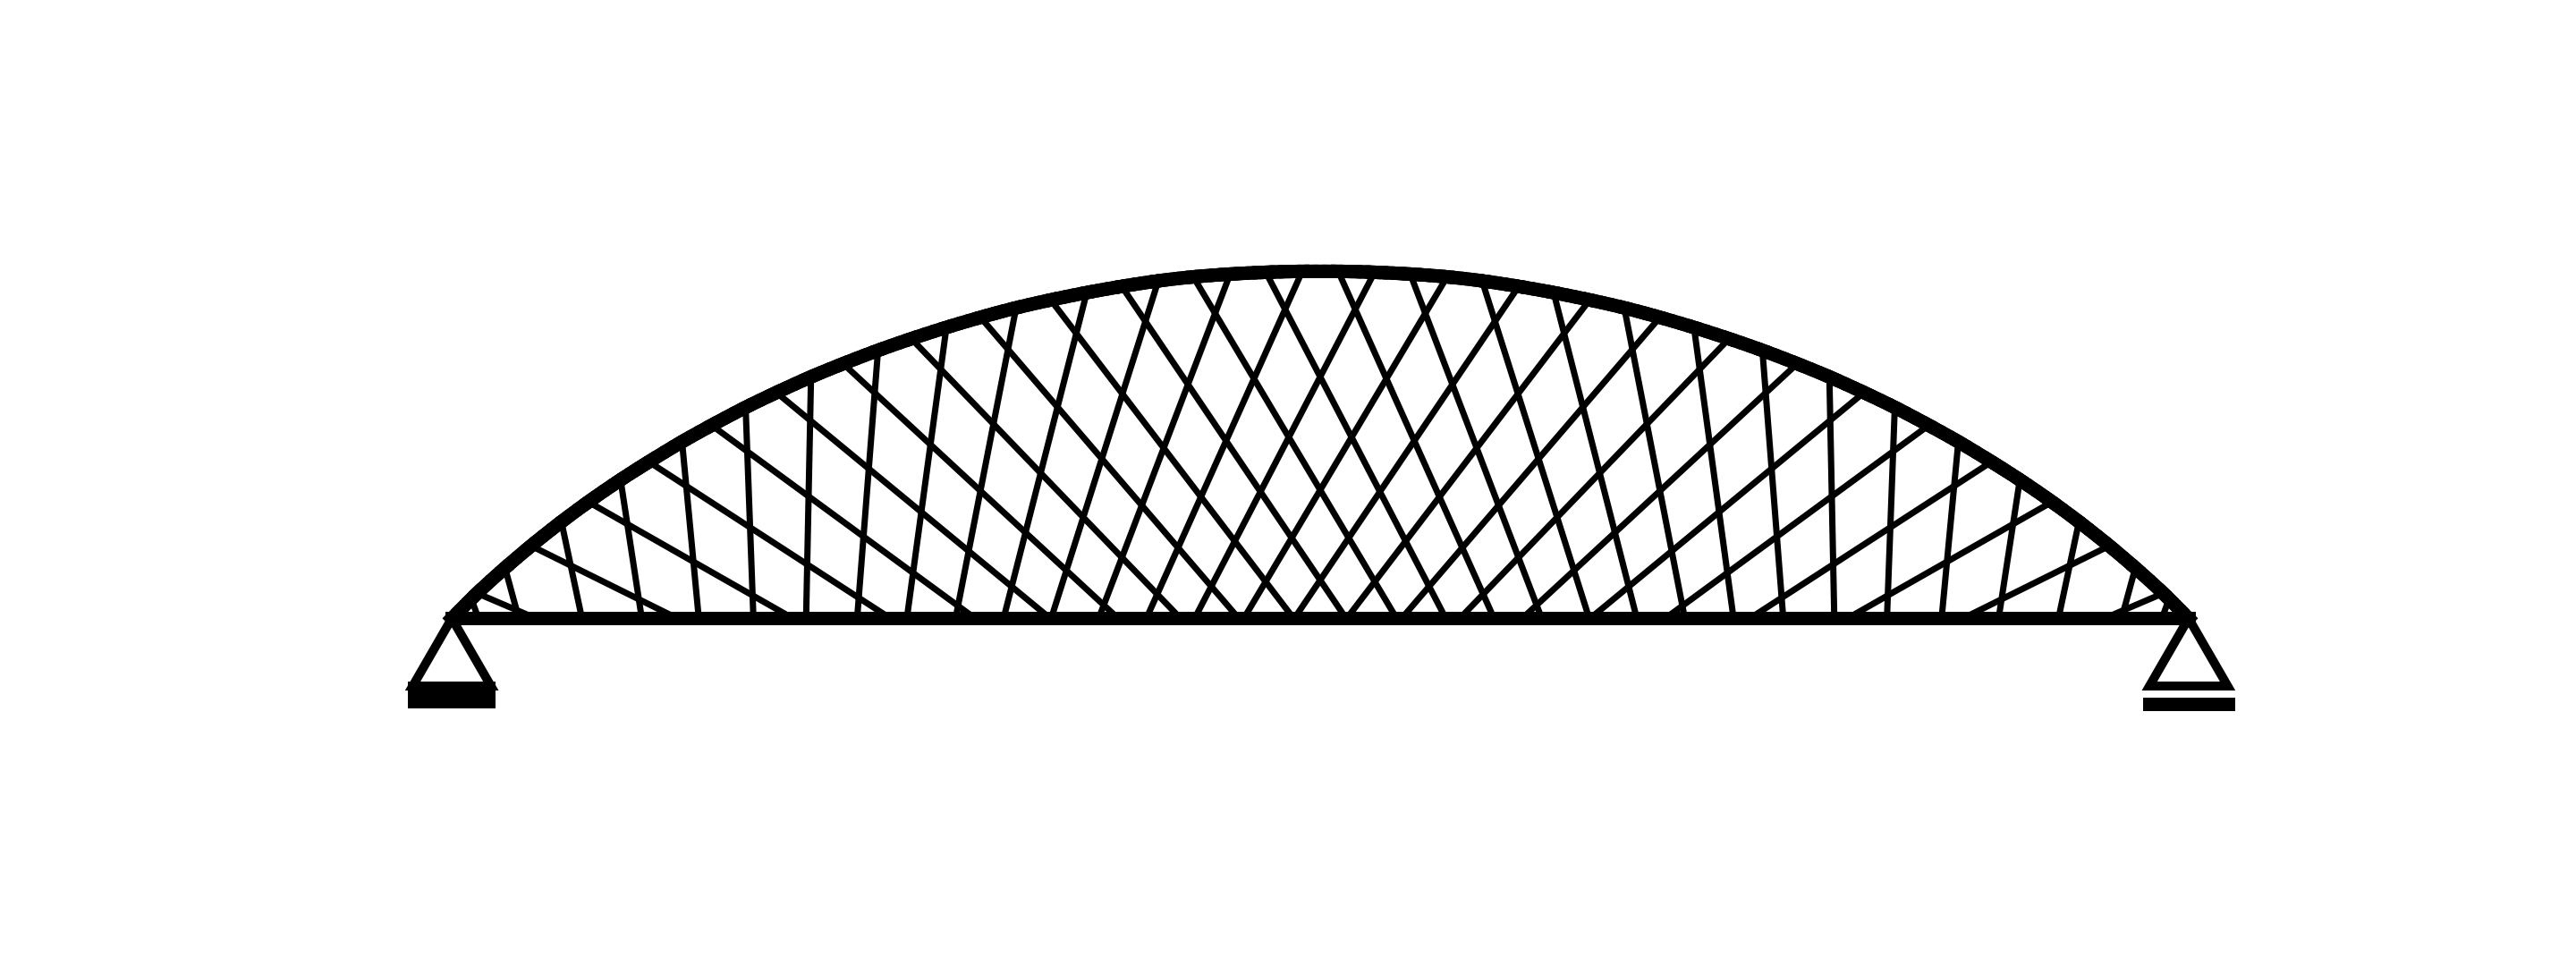
\includegraphics[trim={0 1cm 0 1cm},clip, width=0.65\textwidth]{calculations/hanger density radial/structure_26_radial.png}
    \caption{Structural model of a radial hanger arrangement with 26 hangers per set}
    \label{fig:structure_26_radial}
\end{figure}

The effects under permanent loads are again obtained from a tie moment optimisation
\cref{fig:hd_permanent_radial}

\begin{figure}[H]
    \centering
    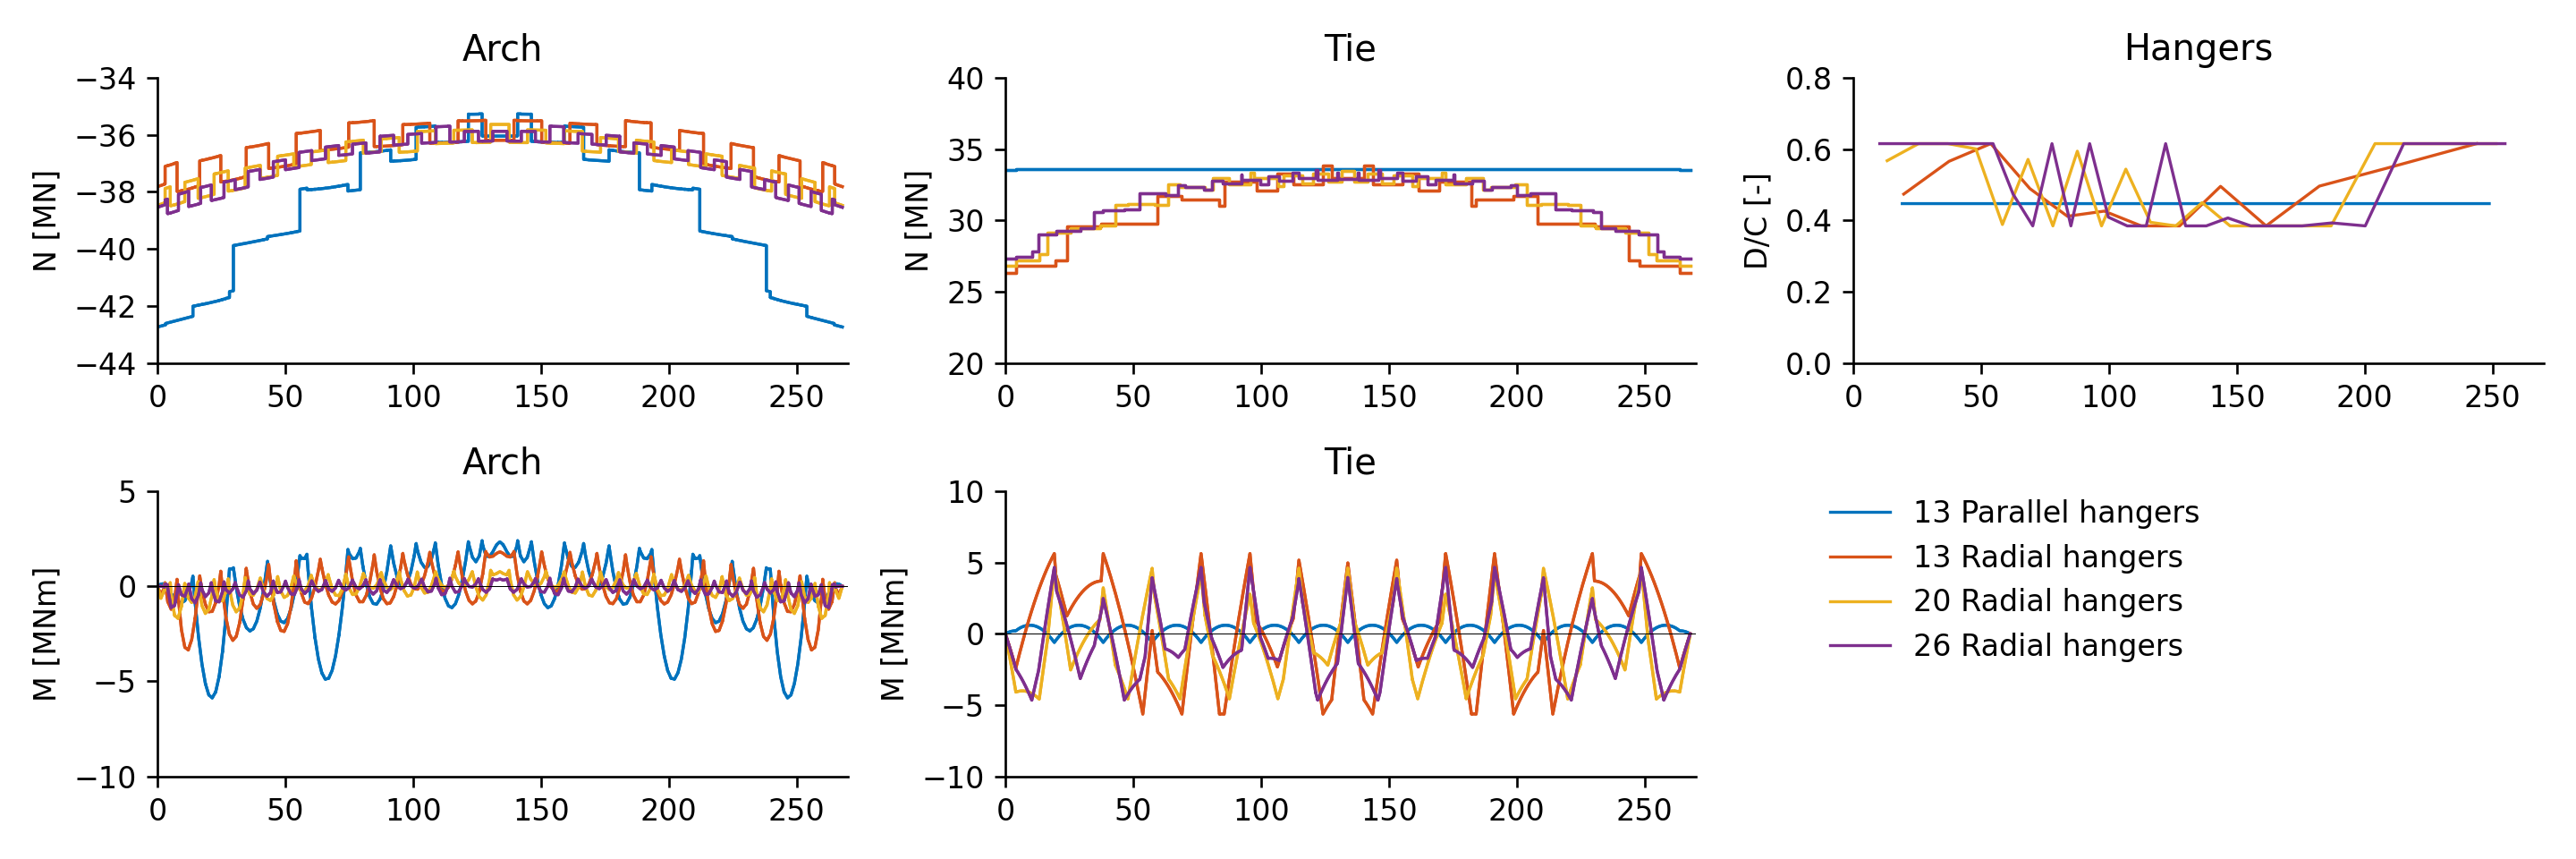
\includegraphics[trim={0 0 0 0},clip, width=0.75\textwidth]{calculations/hanger density radial/permanent.png}
    \caption{Optimised permanent effects for different hanger densities}
    \label{fig:hd_permanent_radial}
\end{figure}

The moment distribution shows the reduction of the shape deviation moment by the constant hanger spacing. All of the radial models are only affected by very weak arch moments independent of the hanger density. The problem with the radial arrangement becomes apparent for the hanger forces. While the parallel arrangement features uniform permanent hanger forces, the radial arrangements show significantly higher forces towards the knuckle. This is due to the non-uniform hanger spacing on the tie girder. Nevertheless, the bending moments in the tie girder cannot be reduced to an acceptable range. The associated complications clearly outweigh the benefits in the moment distribution in the arch. Therefore, the radial arrangement is not further considered. However, it has to be noted that it might prove advantageous with a denser floor beam spacing or a composite deck system.


\section{Floor beam density} \label{sec:floor_beam_density}
It was seen in the previous chapter, that it is impossible to obtain an optimised design with more hangers per set than floor beams. To facilitate the design verifications in the extreme event of cable loss, a denser hanger arrangement has to be paired with a higher floor beam density. It seems a particularly reasonable step, as the Blennerhassett Island Bridge holds the record for hanger spacing on the tie girder at \SI{20}{m}. This was only feasible as the extreme event of floor beam loss was not considered in the design. However, there are other causes to investigate the floor beam and hanger density. Besides the previously mentioned improved behaviour under cable loss and smaller deviations of the arch from the thrust line, a general more continuous transfer of loads might benefit. \medskip

Theoretically, an adapted floor beam spacing changes the entire deck system and its weight. However, the deck is not subject to this investigation, and it is therefore assumed, that the weight of the deck system and the floor beams are constant and independent of the floor beam spacing. Four models with different floor beam and hanger densities are investigated in this section. Besides the final design with 13 floor beams, models with 10, 20 and 27 floor beams are investigated. As an advantage for the sparse model with 10 floor beams, the actual thrust line is assumed as the arch shape (indicated by *). For the other models, the thrust line is approximated by the quartic polynomial with $b=0.962$ as recommended in \cref{sec:arch_shape}. The permanent effects, shown in \cref{fig:fb_permanent}, are obtained by the tie moment optimisation. However, the zero-displacement method also yields very similar results in this case.

\begin{figure}[H]
    \centering
    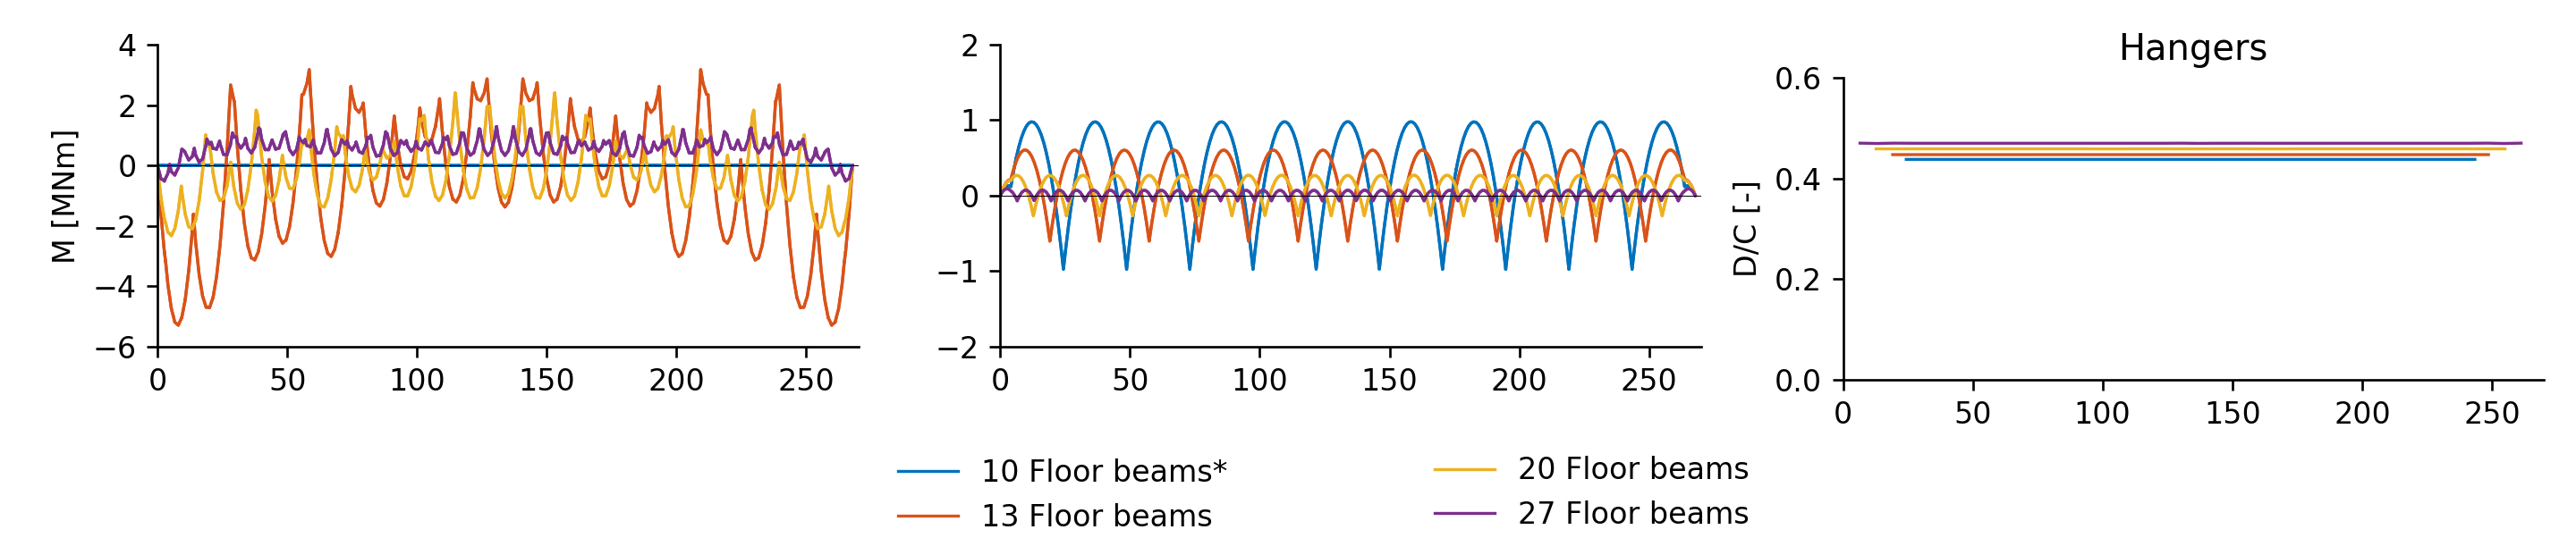
\includegraphics[trim={0 0 1cm 0},clip, width=\textwidth]{calculations/floor beam density/permanent_plot.png}
    \caption{Optimised permanent effects for different floor beam densities}
    \label{fig:fb_permanent}
\end{figure}


All models retain the characteristic permanent effects resulting from the tie optimisation, which are the uniform hanger forces and a uniform tie moment distribution with peaks at $M=\pm\,g_{Tie} \cdot l^2 / 16$. It can be seen that the hanger forces slightly increase, as less weight of the deck is directly carried by the floor beam at the knuckle.
The permanent arch moments for 13 floor beams seem significant in comparison. However, it is known from the arch shape investigation that the moments only lower the D/C ratio by about 0.05. Therefore, none of the models is particularly disadvantageous. Further, the elastic response under characteristic live loading is shown in \cref{fig:fb_live}. 

\begin{figure}[H]
    \centering
    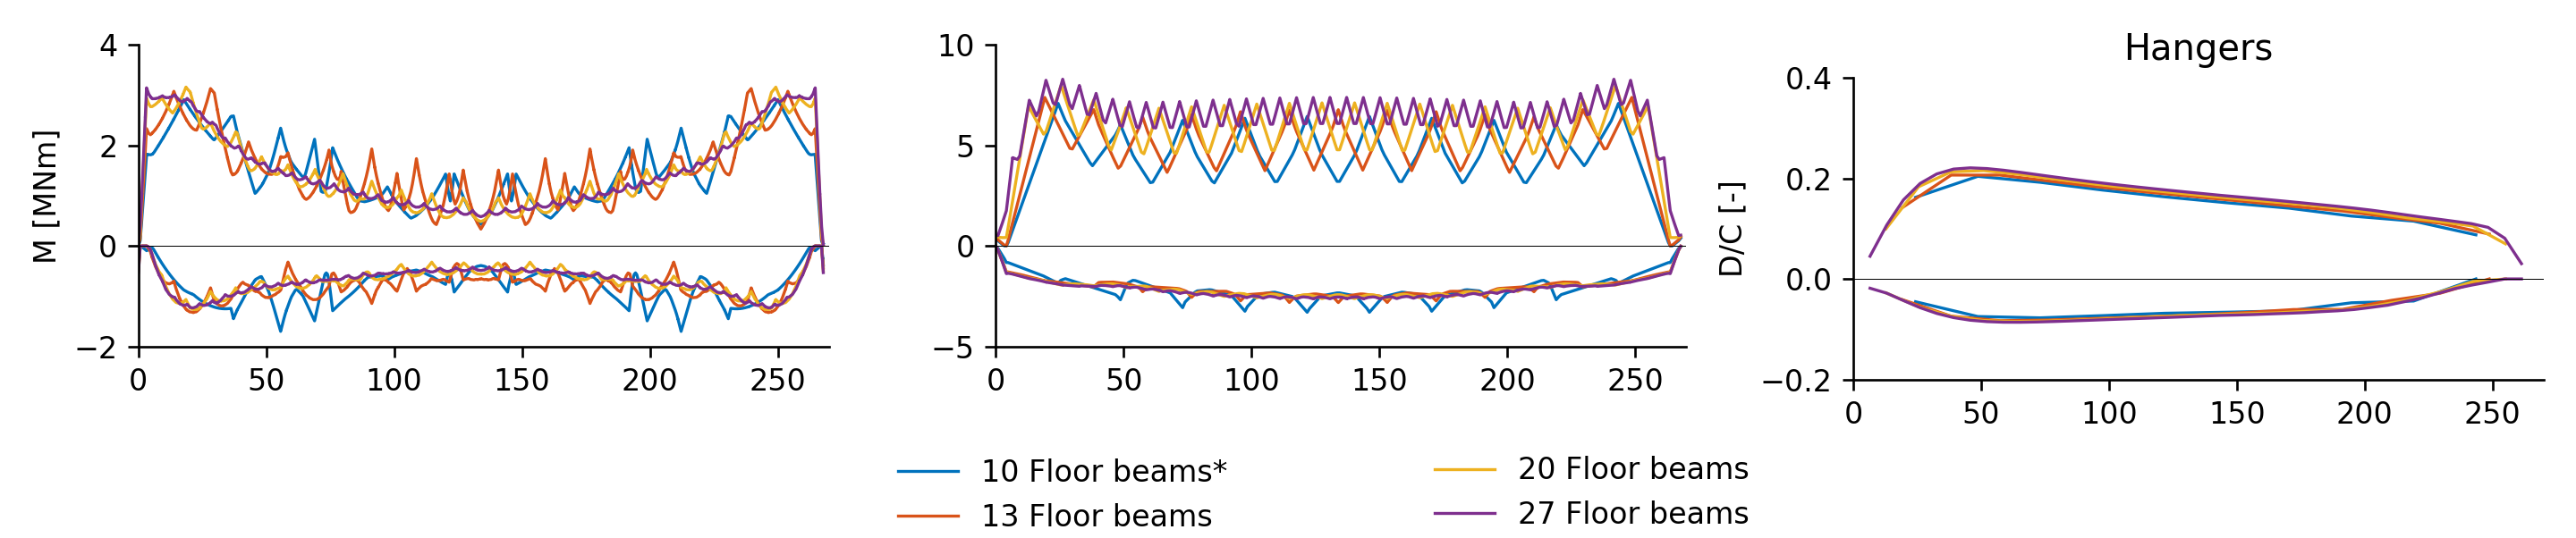
\includegraphics[trim={0 0 1cm 0},clip, width=\textwidth]{calculations/floor beam density/live loading_plot.png}
    \caption{Elastic effects under live loading for different floor beam densities}
    \label{fig:fb_live}
\end{figure}

For the hangers, the response is practically unchanged. Only the hangers very close to the knuckle undergo a lower normal force, as the tie girder at the knuckle carries the corresponding load directly. For the tie girder, the moment effects increase with the floor beam density and constitute a slightly impairing impact on the design verifications. The stronger moments are due to the weaker coupling of the tie and the arch at the floor beams. While the force at the floor beams for the distributed lane load decreases, the force due to the design trucks remains the same. The hanger forces and the bending moments in the tie girder slightly increase due to the equal concentrated force, which is opposed by fewer hangers. The moment distribution on the arch rib shows a different tendency. Overall the effects of the models resemble a similar shape. However, for fewer floor beams, certain moment peaks due to the stronger hanger forces become apparent. To put these differences into the context of the design verifications, the resulting demand over capacity ratios are shown in \cref{tab:fb_dc}.

\begin{table}[H]
    \centering
    \resizebox{0.9\columnwidth}{!}{%
    \input{calculations/floor beam density/dc comparison.txt}
    }
    \caption{Design verifications for different floor beam densities}
    \label{tab:fb_dc}
\end{table}

The extreme event of cable loss is well controlled by a denser hanger arrangement, as observed in the previous chapter. The impacts on the other design verification are comparably small. Both the hangers and the tie girder are affected by a slight increase of about 0.05 in the D/C ratio due to the higher effects under live loading. The effect ranges for the strength-I limit state are shown in \cref{fig:fb_strength} for further details. Considering the arch, 10 floor beams with an optimised shape or 27 floor beams show a well balanced moment distribution. Hence, if it was not for the governing cable loss extreme event, also fewer floor beams do not have a drastic impact on the verifications if the arch shape is adapted to the permanent thrust line.

\begin{figure}[H]
    \centering
    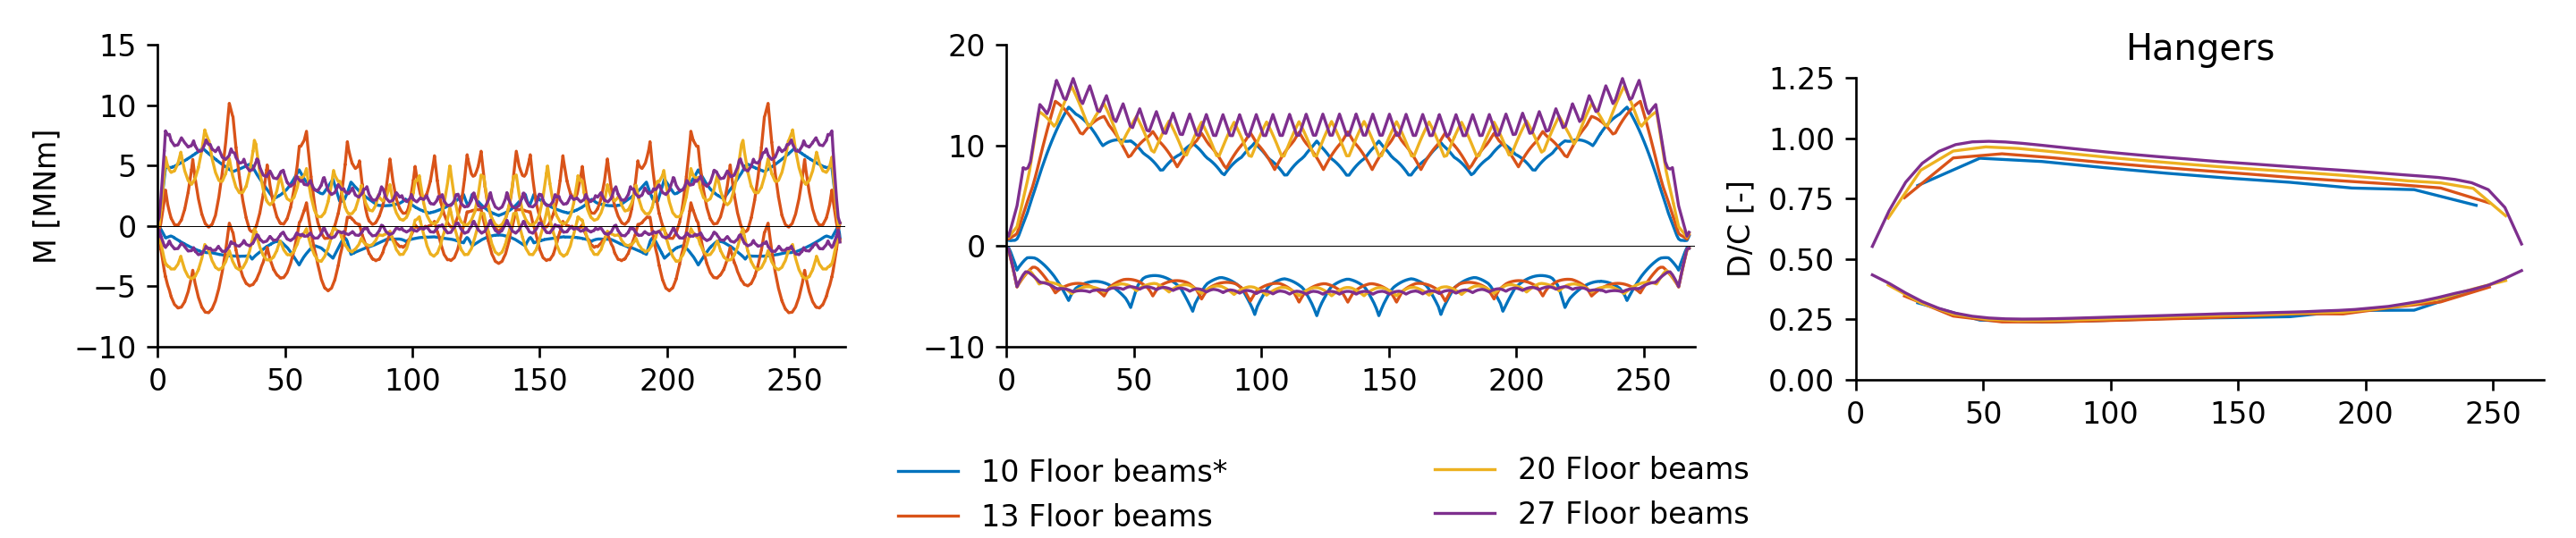
\includegraphics[trim={0 0 1cm 0},clip, width=\textwidth]{calculations/floor beam density/strength-I_plot.png}
    \caption{Effect range for Strength-I limit state for different floor beam densities}
    \label{fig:fb_strength}
\end{figure}


The estimated costs depending on the number of floor beams are shown in \cref{fig:fb_costs}. It is clearly governed by the demand resulting from cable loss. Whereas for the tie, the extreme event is well controlled with 10 floor beams, it takes about 25 floor beams for the arch to eradicate the respective demands completely. Further, only minor changes in costs are observed. The cost of the hangers and the tie increase slightly due to the slightly unfavourable behaviour under live loading. Ultimately, the purple line can be shifted to the left side by a detailed analysis of the dynamic amplification factors. It also moves the optimum to the left side, which was the case for the Blennerhassett Island Bridge. Therefore, there this no optimisation potential with respect to the aspect of the floor beam density.

\begin{figure}[H]
    \centering
    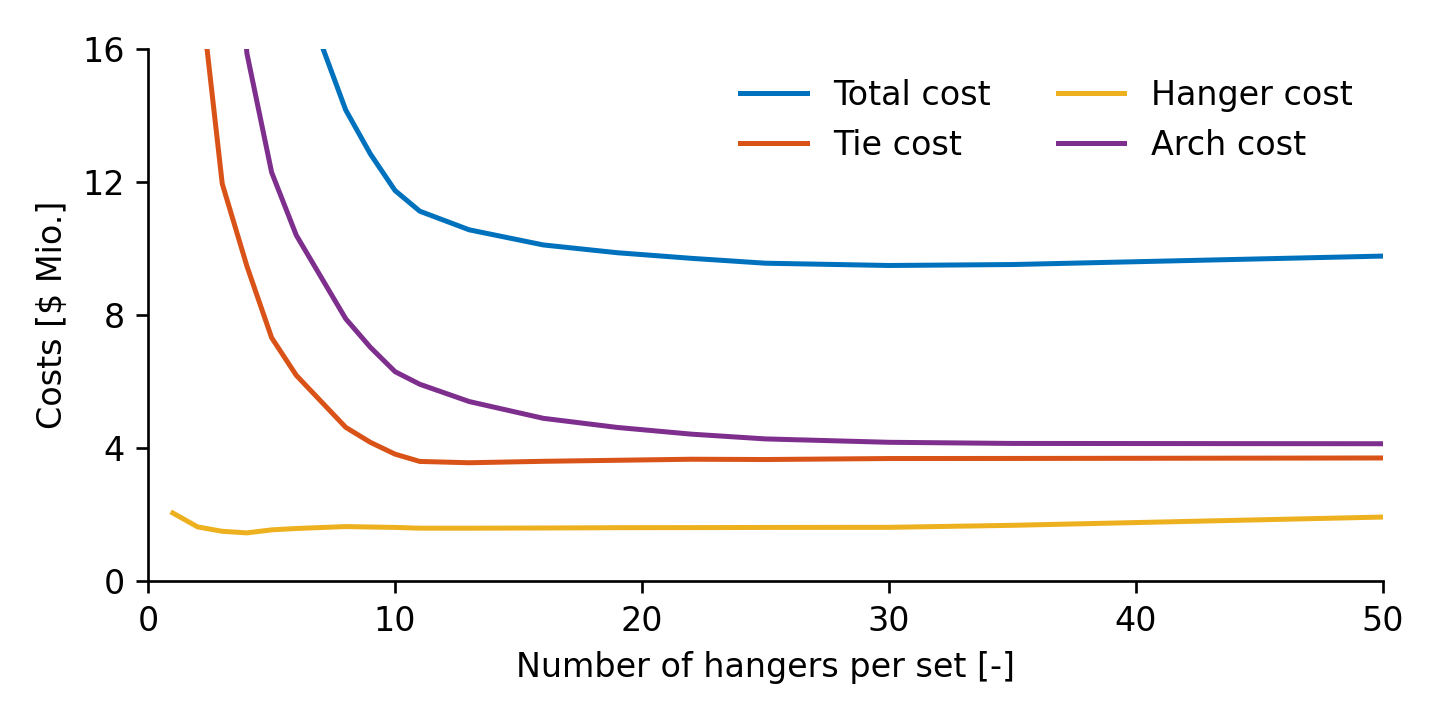
\includegraphics[width=0.7\textwidth]{calculations/floor beam density/cost comparison.png}
    \caption{Estimated costs for different floor beam densities}
    \label{fig:fb_costs}
\end{figure}


\newpage
\section{Hanger inclination} \label{sec:inclination}
The investigation in this section focuses on the hanger arrangements' main characteristic, the hanger inclination. First, the parallel hanger arrangement is investigated in \cref{sec:parallel}. Further, variable hanger inclinations are also considered. Therefore, the constant change of inclination arrangement is investigated in \cref{sec:constant_change} for further optimisation potential. Ultimately, a numerical optimisation of an unpatterned hanger arrangement is conducted in \cref{sec:unpatterned} as a comparison to the common hanger arrangement patterns.


\subsection{Parallel hanger arrangement}\label{sec:parallel}
In the previous sections, the inclination has been left at \SI{64}{\degree} as in the final design of the Blennerhassett Island Bridge. This choice is critically assessed by the investigation of models with inclinations from \SI{45}{\degree} to \SI{85}{\degree}. The first part focuses on their elastic response to the characteristic load cases and the internal forces under permanent loads.  In the second part, the implications on the design verification and the estimated costs are examined. 
 
\subsubsection{Characteristic behaviour}
The investigation of the arch shape in Section \ref{sec:arch_shape}, showed that the spacing of the hanger anchorage nodes on the arch rib has a significant impact on the internal forces for the considered design. By changing the inclination of the hangers the respective spacing changes rather randomly. The arch shapes are taken as the respective thrust lines of each arrangement to exclude these random implications in this investigation of the hanger inclination. Hence, the permanent moment distributions disappear for all models. Also, the permanent moment distribution on the tie girder resulting from the tie moment minimisation is identical for all models at $M_{p,Tie}=\pm \SI{650}{kNm}$. The other permanent internal forces are shown in \cref{fig:inclination_permanent}.

\begin{figure}[H]
    \centering
    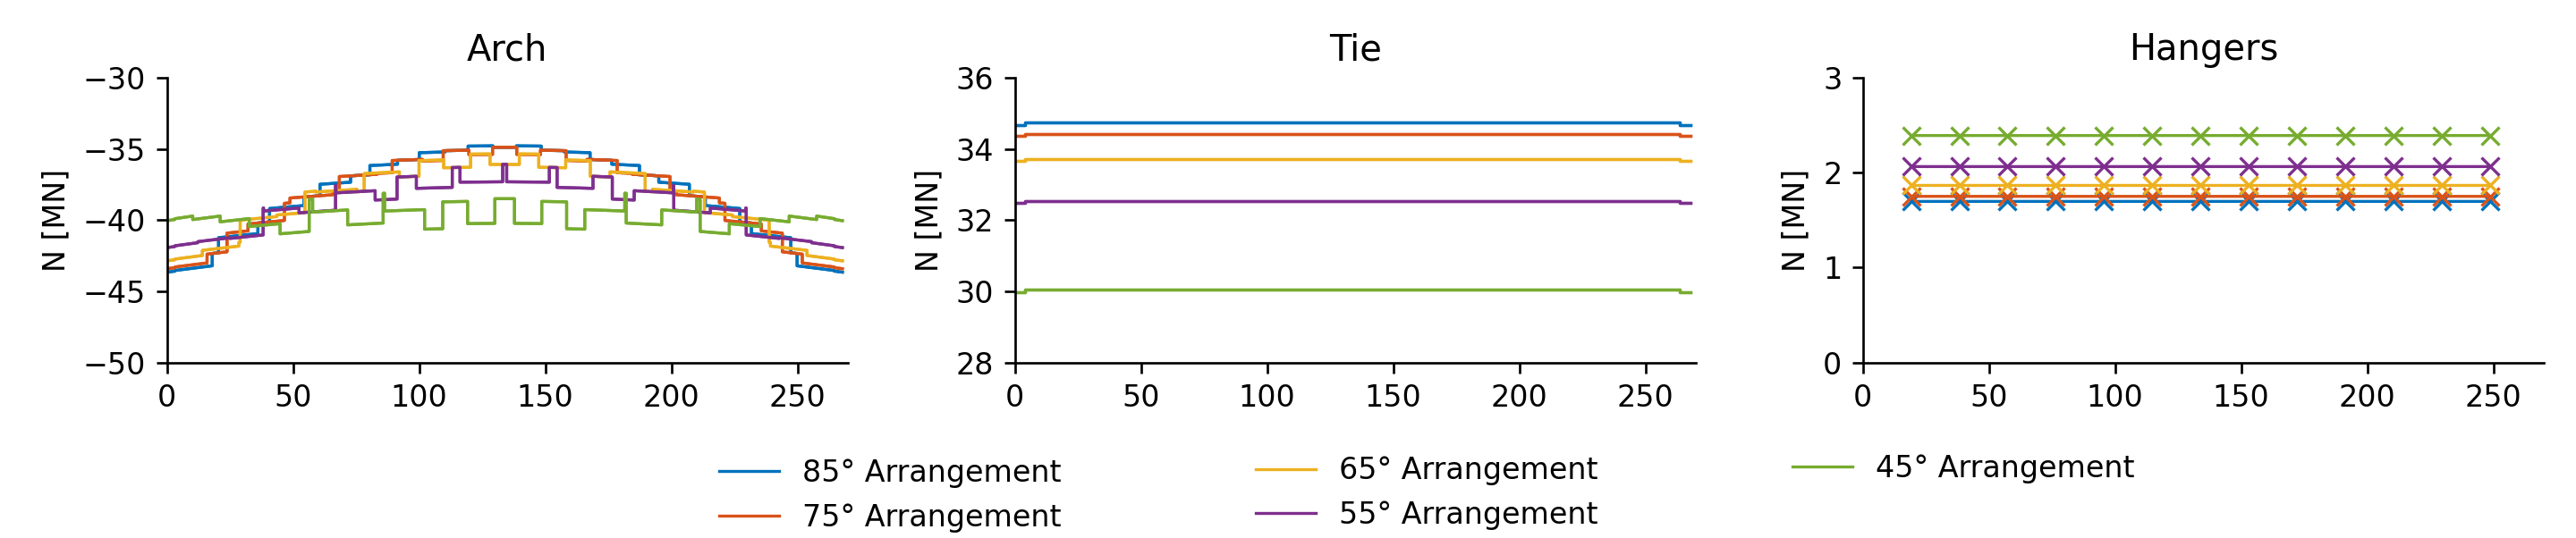
\includegraphics[trim={1cm 0 1cm 0},clip, width=\textwidth]{calculations/parallel arrangement comparison/permanent_plot.png}
    \caption{Permanent internal forces for different hanger inclinations}
    \label{fig:inclination_permanent}
\end{figure}

The permanent hanger forces increase for flatter hanger inclinations due to the smaller vertical component of the respective force. They are still uniform for each model and cause no change in the normal force distribution in the tie girder. For the normal forces in the arch, a relatively uniform distribution is observed for the \SI{45}{\degree} arrangement. For the respective continuous hanger arrangement, it was seen in \cref{sec:arch_shape}, that its thrust line resembles a circle and the hanger forces on the arch are oriented radially. Therefore, the direction of the resulting normal force changes, the magnitude remains the same, however. Its lower normal force at the knuckle can alternatively be explained by the circle's steeper inclination, which approximates the thrust line of the flat arrangements. As the vertical component of the normal force in the arch is roughly the same for all models, the total normal force is smaller for steep arch shapes at the knuckle. Conversely, the \SI{45}{\degree} arrangement causes a higher normal force in the crown of the arch. This high normal force is due to the horizontal force components in the hangers, which reduces the structure's global lever arm and tension in the tie. 
A similar elastic response is observed for the characteristic dead loading, shown in \cref{fig:inclination_dead}.
\begin{figure}[H]
    \centering
    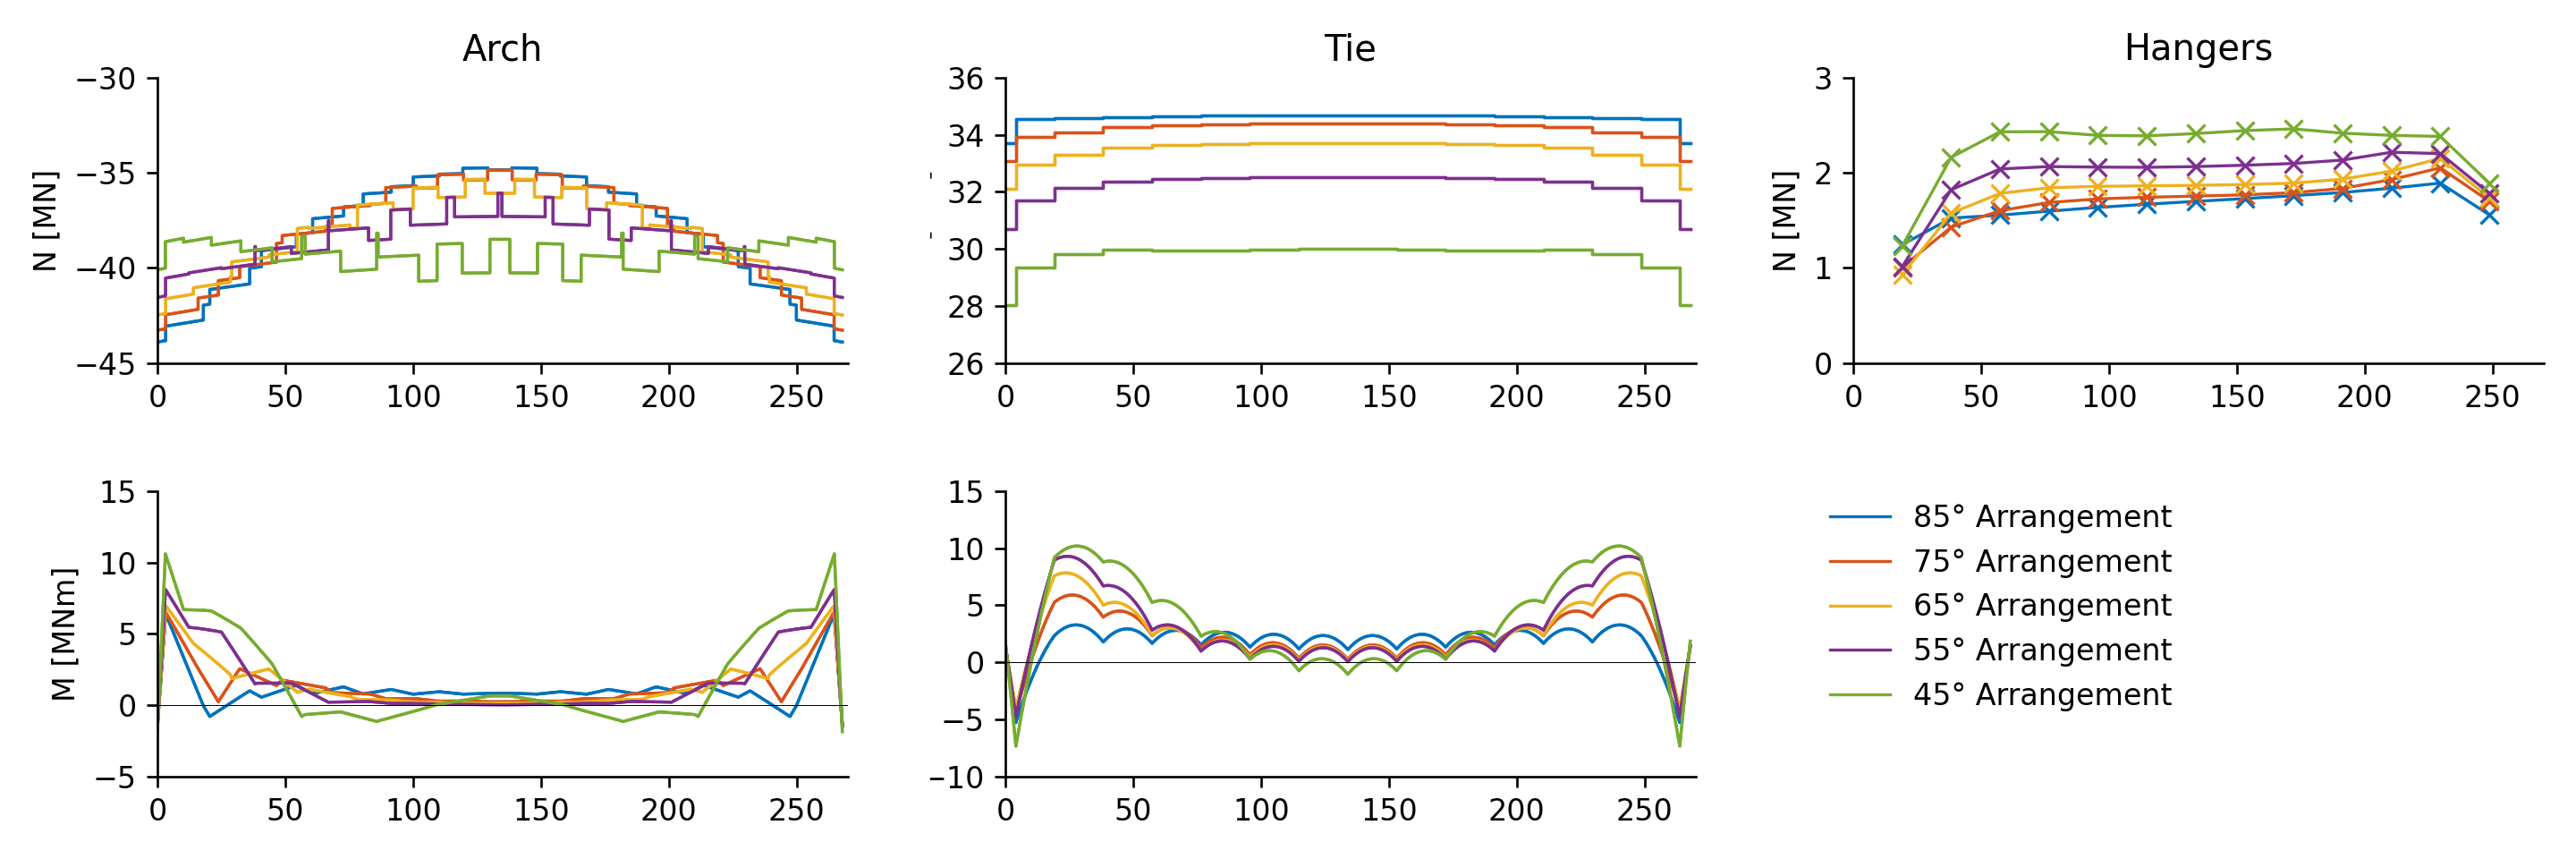
\includegraphics[width=\textwidth]{calculations/parallel arrangement comparison/dead load_plot.png}
    \caption{Elastic responses to dead loading for different hanger inclinations}
    \label{fig:inclination_dead}
\end{figure}

Most hanger forces are in a similar range as for the optimised permanent state. This is due to the uniform embedding of the tie girder in the field yielding uniform hanger forces. Therefore, also the normal forces of the arch and the tie show a similar shape as was seen for the permanent state. However, in the knuckle area, large bending moments are observed for flat inclinations. Their cause is the lack of stiffness between the arch and the tie in this region, leaving them to carry the loads on bending. This lack of stiffness becomes evident from the respective hanger arrangements presented in \cref{fig:arrangements}.

\begin{figure}[H]
\centering
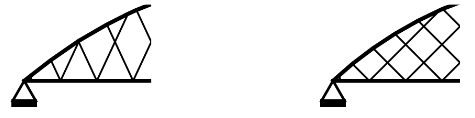
\includegraphics[width=0.5\textwidth]{overleaf/Pictures/snap_knuckle.PNG}
\caption{Knuckle regions of the $\alpha=65\degree$ and  $\alpha=45\degree$ arrangements}
\label{fig:arrangements}
\end{figure}

The \SI{45}{\degree} arrangement features only hangers from one set in the knuckle region, which attach almost perpendicular to the arch. The stiffness of this arrangement is therefore much lower than the one of the \SI{65}{\degree} arrangement, which has more connections and also more suitable hanger inclinations. Further, the elastic response range to live loading is presented in \cref{fig:inclination_live}.

\begin{figure}[H]
    \centering
    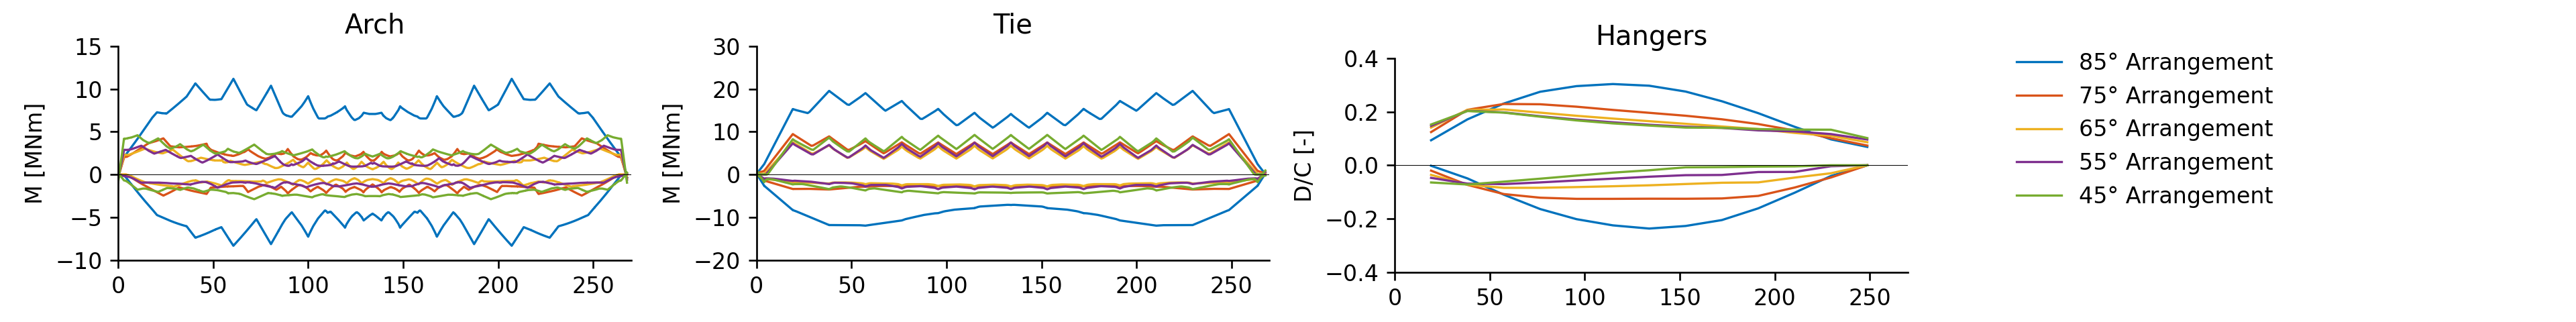
\includegraphics[trim={1cm 0 1cm 0},clip, width=\textwidth]{calculations/parallel arrangement comparison/live loading_plot.png}
    \caption{Elastic response ranges to live loading loading for different hanger inclinations}
    \label{fig:inclination_live}
\end{figure}

For live loading, it is the steepest arrangement which is affected by the largest internal force effects. Especially its hanger force shows a unique behaviour with the ones in the middle carrying the largest forces. As the hangers are less interconnected with each other, the coupling of the arch and the tie is generally lower. Therefore, the \SI{85}{\degree} arrangement is affected by larger bending moments, as the efficient truss action is not formed. Further, this increases the characteristic length of the embedded tie girder, which especially causes the middle hanger to be affected by large forces. There can also be strong compressive forces for the considered hanger, which implicates the danger of hanger unloading. However, it has to be considered that the steep hanger arrangement utilises a shorter total hanger length, which poses an upside opposing the observed disadvantages. Within the other four studied models, the differences are much lower. Still, it is indicated by the lower moment distributions for the \SI{55}{\degree} and the \SI{65}{\degree} arrangements, that a stronger truss action is formed in the respective cases. It can be concluded, that neither a steep nor a flat hanger arrangement forms an adequate coupling of the arch rib and the tie girder. 
Ultimately, the effects for the event of losing the fourth cable are shown in \cref{fig:inclination_cable} to represent the characteristic behaviour under cable loss.

\begin{figure}[H]
    \centering
    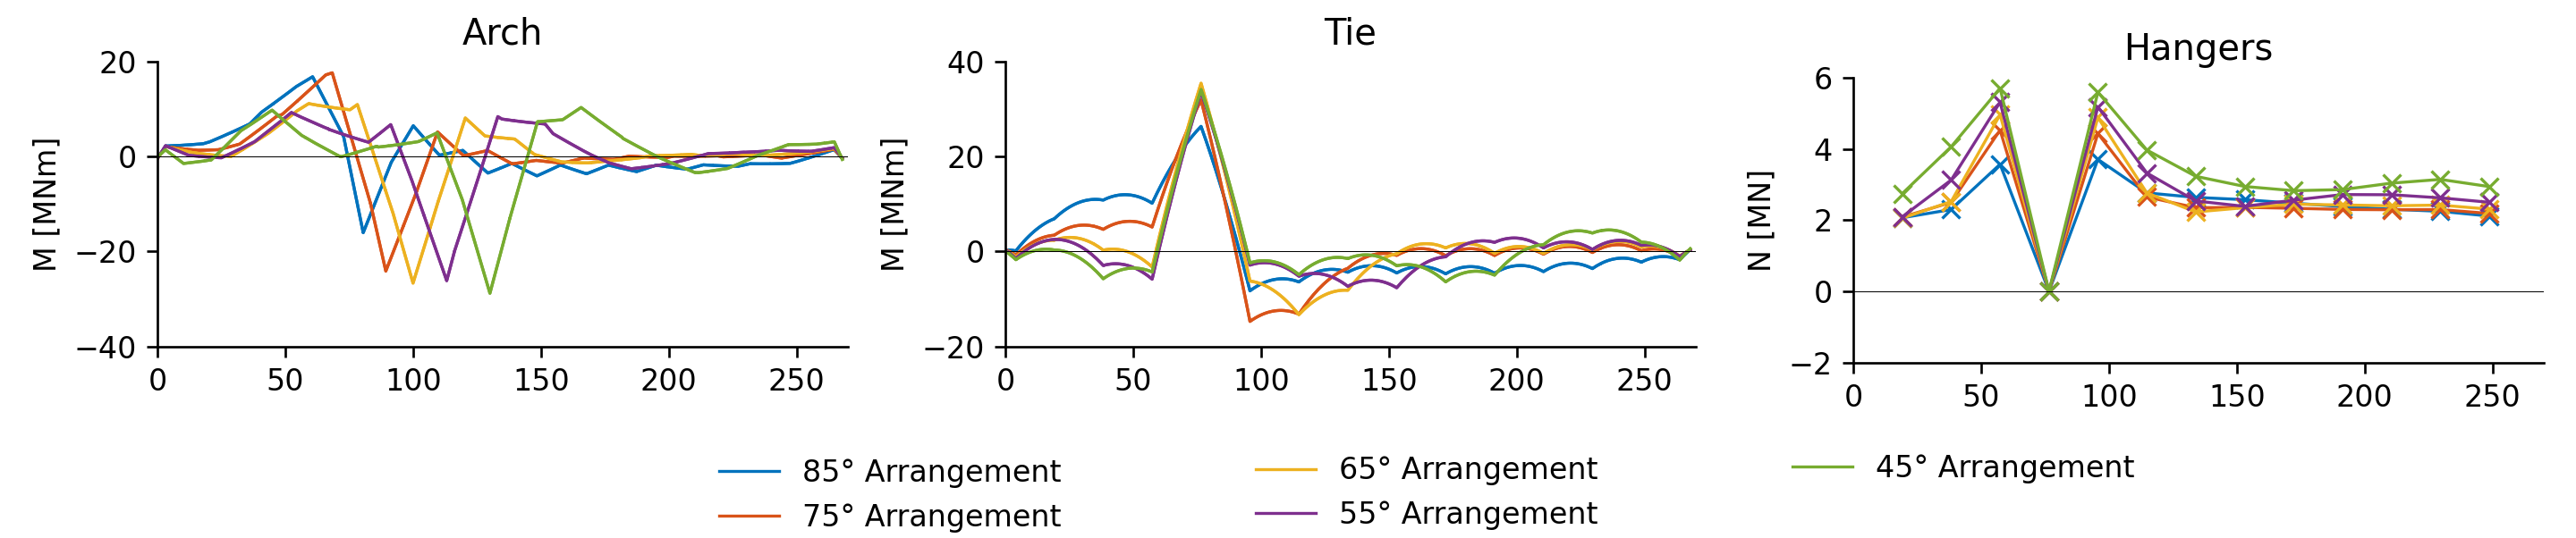
\includegraphics[trim={1cm 0 1cm 0},clip, width=\textwidth]{calculations/parallel arrangement comparison/cable loss 4_plot.png}
    \caption{Approximated dynamic response to the loss of the fourth hanger for different hanger inclinations}
    \label{fig:inclination_cable}
\end{figure}

The extreme event of cable loss shows the opposite preference. Because of the generally lower permanent hanger forces and the weaker coupling, the steep arrangements result in lower demands compared to the flat inclinations. Further, the similar directions of the two hanger sets allow them to distribute the lost cable forces better. 

\subsubsection{Design verifications and costs}
To conclude the previous observations, the deciding demand over capacity ratios are shown for each model and each segment in Table \ref{tab:dc_inclination}.

\begin{table}[H]
    \centering
    \caption{Maximum demand over capacity ratios for different hanger inclinations}
    \label{tab:dc_inclination}
    \resizebox{0.9\columnwidth}{!}{%   
    \begin{tabular}{lccccccc}
    \hline
    Model & \multicolumn{7}{c}{Demand / Capacity} \\
     & Arch 1 & Arch 2 & Arch 3 & Tie 1 & Tie 2 & Tie 3 & Hangers \\ \hline
    85\degree Arrangement & 0.84 (S3) & 1.04 (CL) & 1.02 (CL) & 0.98 (TF) & 1.28 (TF) & 1.19 (TF) & 1.13 (FA) \\ 
    75\degree Arrangement & 0.83 (S3) & 1.10 (CL) & 1.06 (CL) & 0.82 (TF) & 1.00 (TF) & 0.95 (TF) & 0.95 (FA) \\ 
    65\degree Arrangement & 0.83 (S3) & 1.14 (CL) & 1.10 (CL) & 0.79 (TF) & 0.95 (TF) & 0.91 (TF) & 0.94 (S1) \\ 
    55\degree Arrangement & 0.84 (CL) & 1.15 (CL) & 1.11 (CL) & 0.76 (TF) & 0.94 (TF) & 0.90 (TF) & 0.99 (CL) \\ 
    45\degree Arrangement & 0.81 (CL) & 1.21 (CL) & 1.19 (CL) & 0.72 (TF) & 0.94 (TF) & 0.90 (TF) & 1.09 (CL) \\ 
    \hline
    \end{tabular}
    }
\end{table}
In the arch segments, a decrease in the demand in the extreme event of cable loss is observed for steeper arrangements. It is mainly due to the significant horizontal components in the flat arrangements. While the normal force under identical vertical components is approximately 40\% greater for the \SI{45}{\degree} arrangement, the demand is approximately 20\% larger, as not the entire demand results from the lost normal force. On the other hand, the verification slightly improves for the first arch segment, due to the lower normal force in the knuckle region. For the tie girder segments, the extreme event of tie fracture remains decisive for all models. The large increase in demand for the steepest arrangement is due to its inefficient behaviour under live loading. Between the other models, it is the lower normal force in the tie girder, which renders the flat arrangement slightly beneficial. For hangers, neither of the extreme arrangements gives an improvement. The steep hanger arrangement suffers from fatigue due to the weak interconnection between the hangers. For the flat arrangement, it is again the cable loss event which causes the highest demands. An optimum demand for the hangers is obtained by the \SI{65}{\degree} and the \SI{75}{\degree} arrangement. Finally, the costs of the investigated models, which are shown in \cref{tab:cost_inclination}, are considered. Correlating to the previous observations, the arch rib's costs can be reduced by steeper arrangements, whereas the tie girder becomes cheaper for flat inclinations. Significant changes are also observed for the hangers' costs, which are optimised for inclinations similar to the final design. Also, the overall costs are minimised for these models. However the optimum range is rather broad from \SI{65}{\degree} to \SI{75}{\degree}.


\begin{table}[H]
    \centering
    \caption{Maximum demand over capacity ratios for different hanger inclinations}
    \label{tab:cost_inclination}
    \resizebox{0.64\columnwidth}{!}{%
    \begin{tabular}{lcccc}
    \hline
    Model & Arch cost & Tie cost & Hanger cost & Total cost \\
     & [\$ Mio.] & [\$ Mio.] & [\$ Mio.] & [\$ Mio.] \\ \hline
    85\degree Arrangement & 5.09 & 4.68 & 1.78 & 11.56 \\ 
    75\degree Arrangement & 5.27 & 3.74 & 1.54 & 10.56 \\ 
    65\degree Arrangement & 5.40 & 3.57 & 1.59 & 10.56 \\ 
    55\degree Arrangement & 5.46 & 3.52 & 1.79 & 10.78 \\ 
    45\degree Arrangement & 5.68 & 3.46 & 2.20 & 11.35 \\ 
    \hline
    \end{tabular}
    }
\end{table}

\subsection{Constant change of inclination arrangement}\label{sec:constant_change}
In the previous section, the steep and the flat arrangements both have shown a specific upside. The constant change of inclination arrangement allows a combination of steep inclinations near the knuckle and medium inclinations in the span. Further, multiple studies have claimed optimality of this arrangement. Therefore, its potential for optimisation is assessed in this section, using models with an average inclination angle of $\alpha_{mid} = 65\degree$. The starting inclination $\alpha_1$ is varied up to a value of $105\degree$. Two of these models are shown in \cref{fig:arrangement_85_45} and \cref{fig:arrangement_105_25}.

\begin{figure}[H]
\centering
\begin{subfigure}{0.5\textwidth}
    \centering
    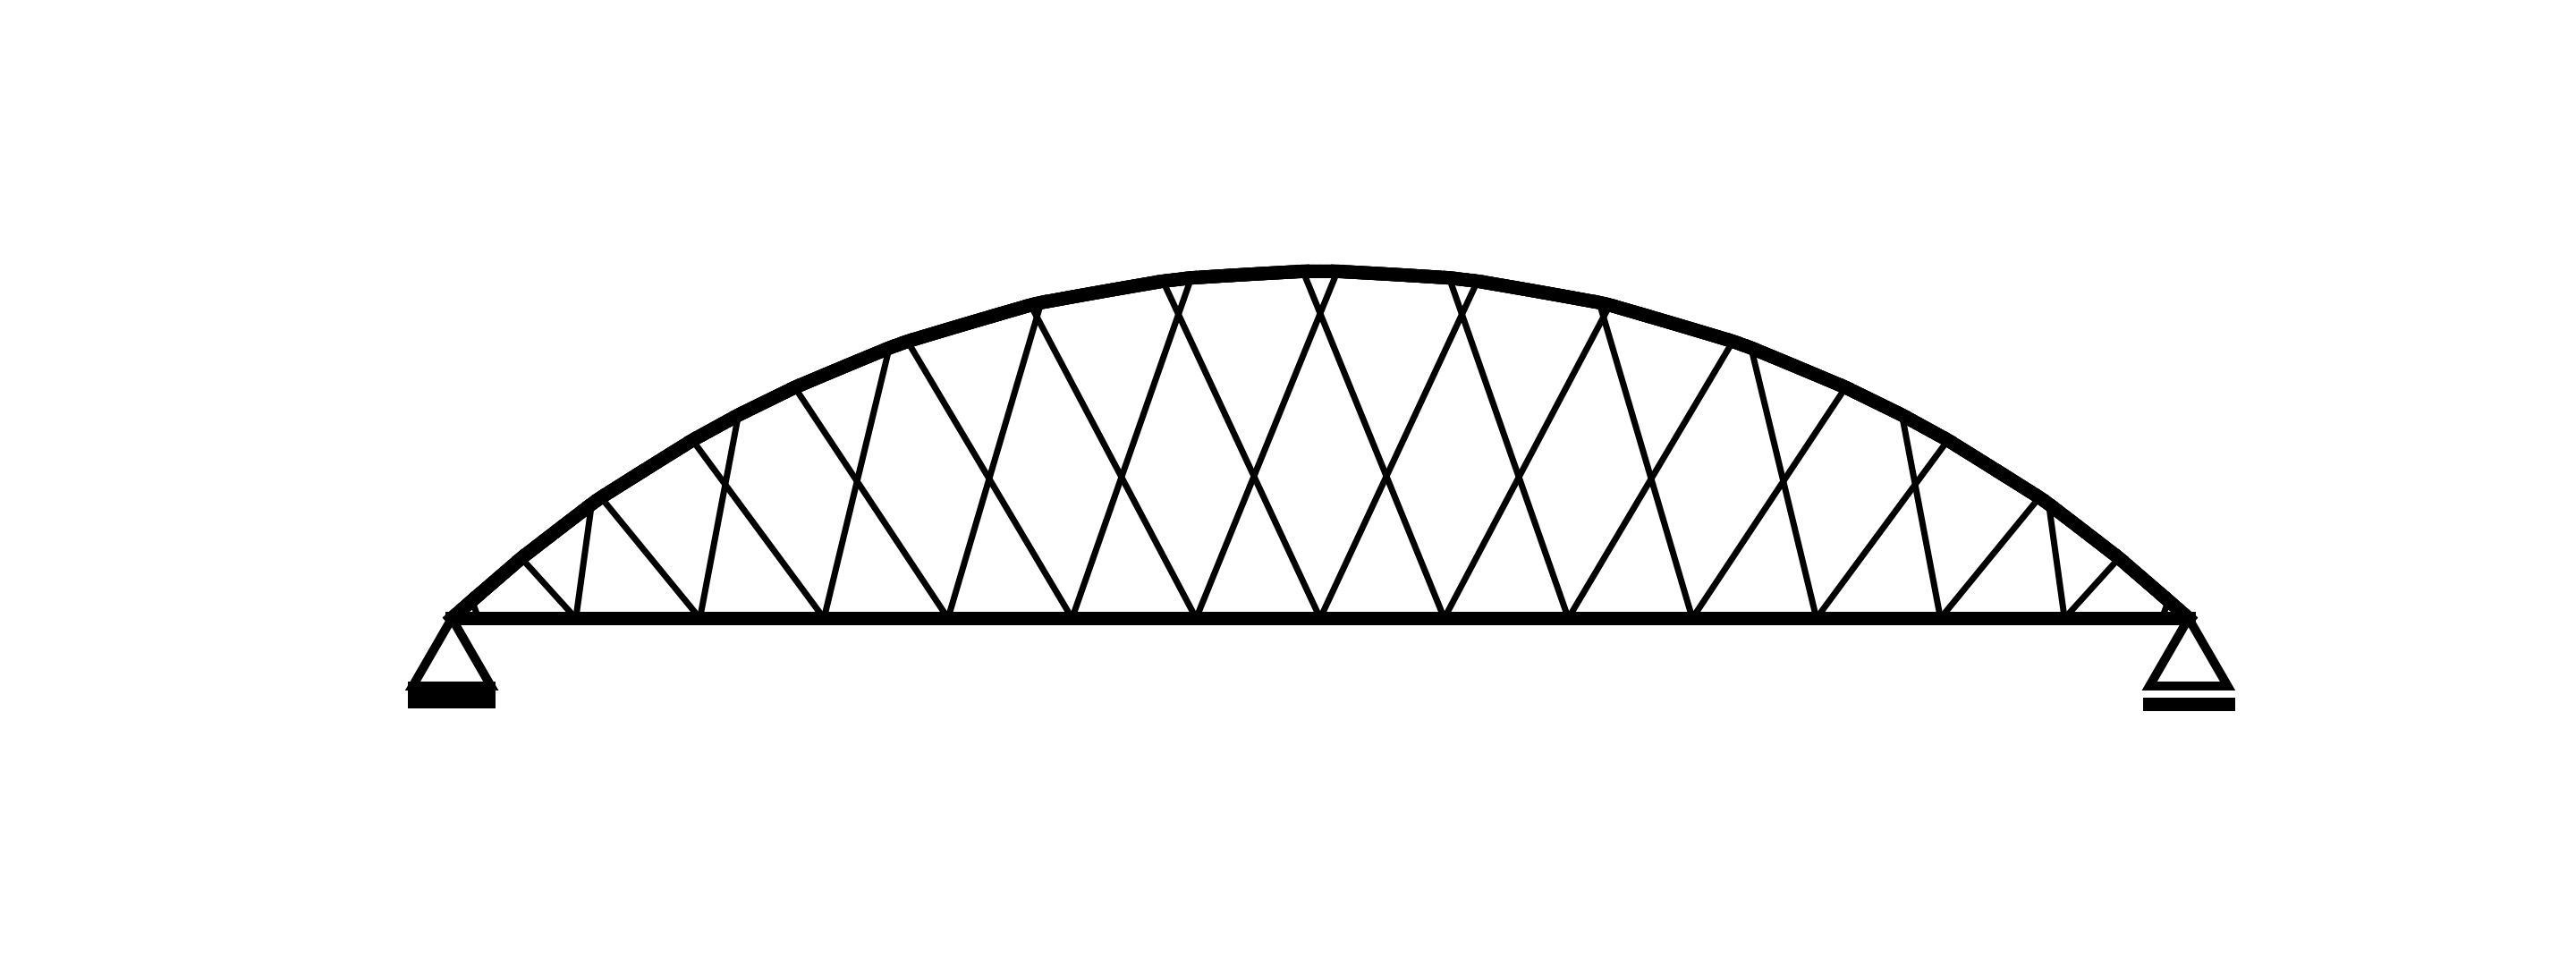
\includegraphics[trim={1.5cm 1cm 1.3cm 1cm},clip, width=0.9\textwidth]{calculations/constant change arrangement/arrangement_85_45.png}
    \caption{$85\degree$ to $45\degree$ arrangement ($\Delta\alpha=3.3\degree$)}
    \label{fig:arrangement_85_45}
\end{subfigure}%
\begin{subfigure}{.5\textwidth}
    \centering
    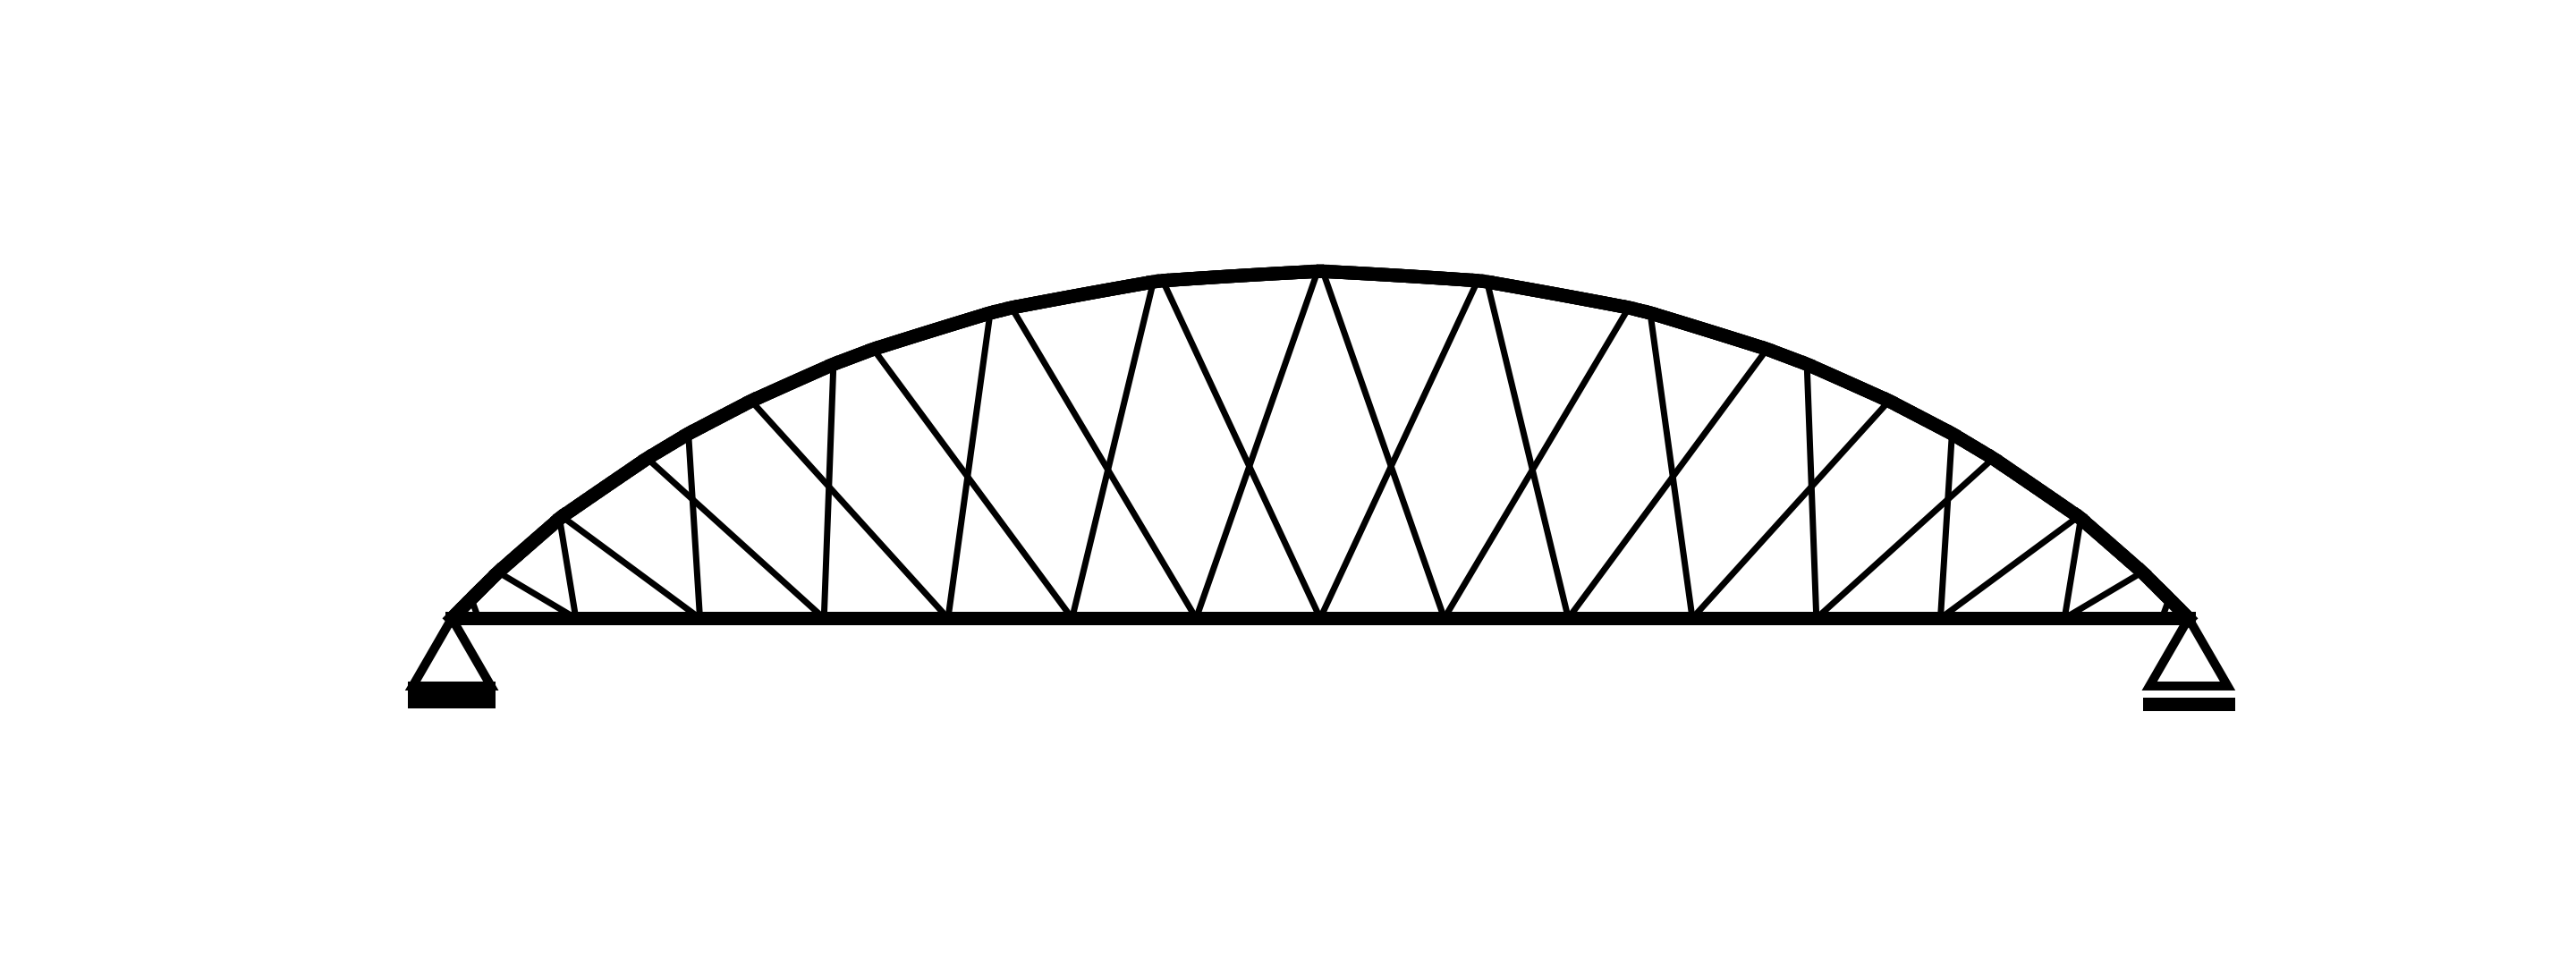
\includegraphics[trim={1.5cm 1cm 1.3cm 1cm},clip, width=0.9\textwidth]{calculations/constant change arrangement/arrangement_105_25.png}
    \caption{$105\degree$ to $25\degree$ arrangement ($\Delta\alpha=6.7\degree)$}
    \label{fig:arrangement_105_25}
\end{subfigure}
\caption{Constant change of inclination arrangements}
\label{fig:constant change arrangements}
\end{figure}

The elastic responses to dead loads indicate the structural behaviour and are presented in \cref{fig:change_live}.

\begin{figure}[H]
    \centering
    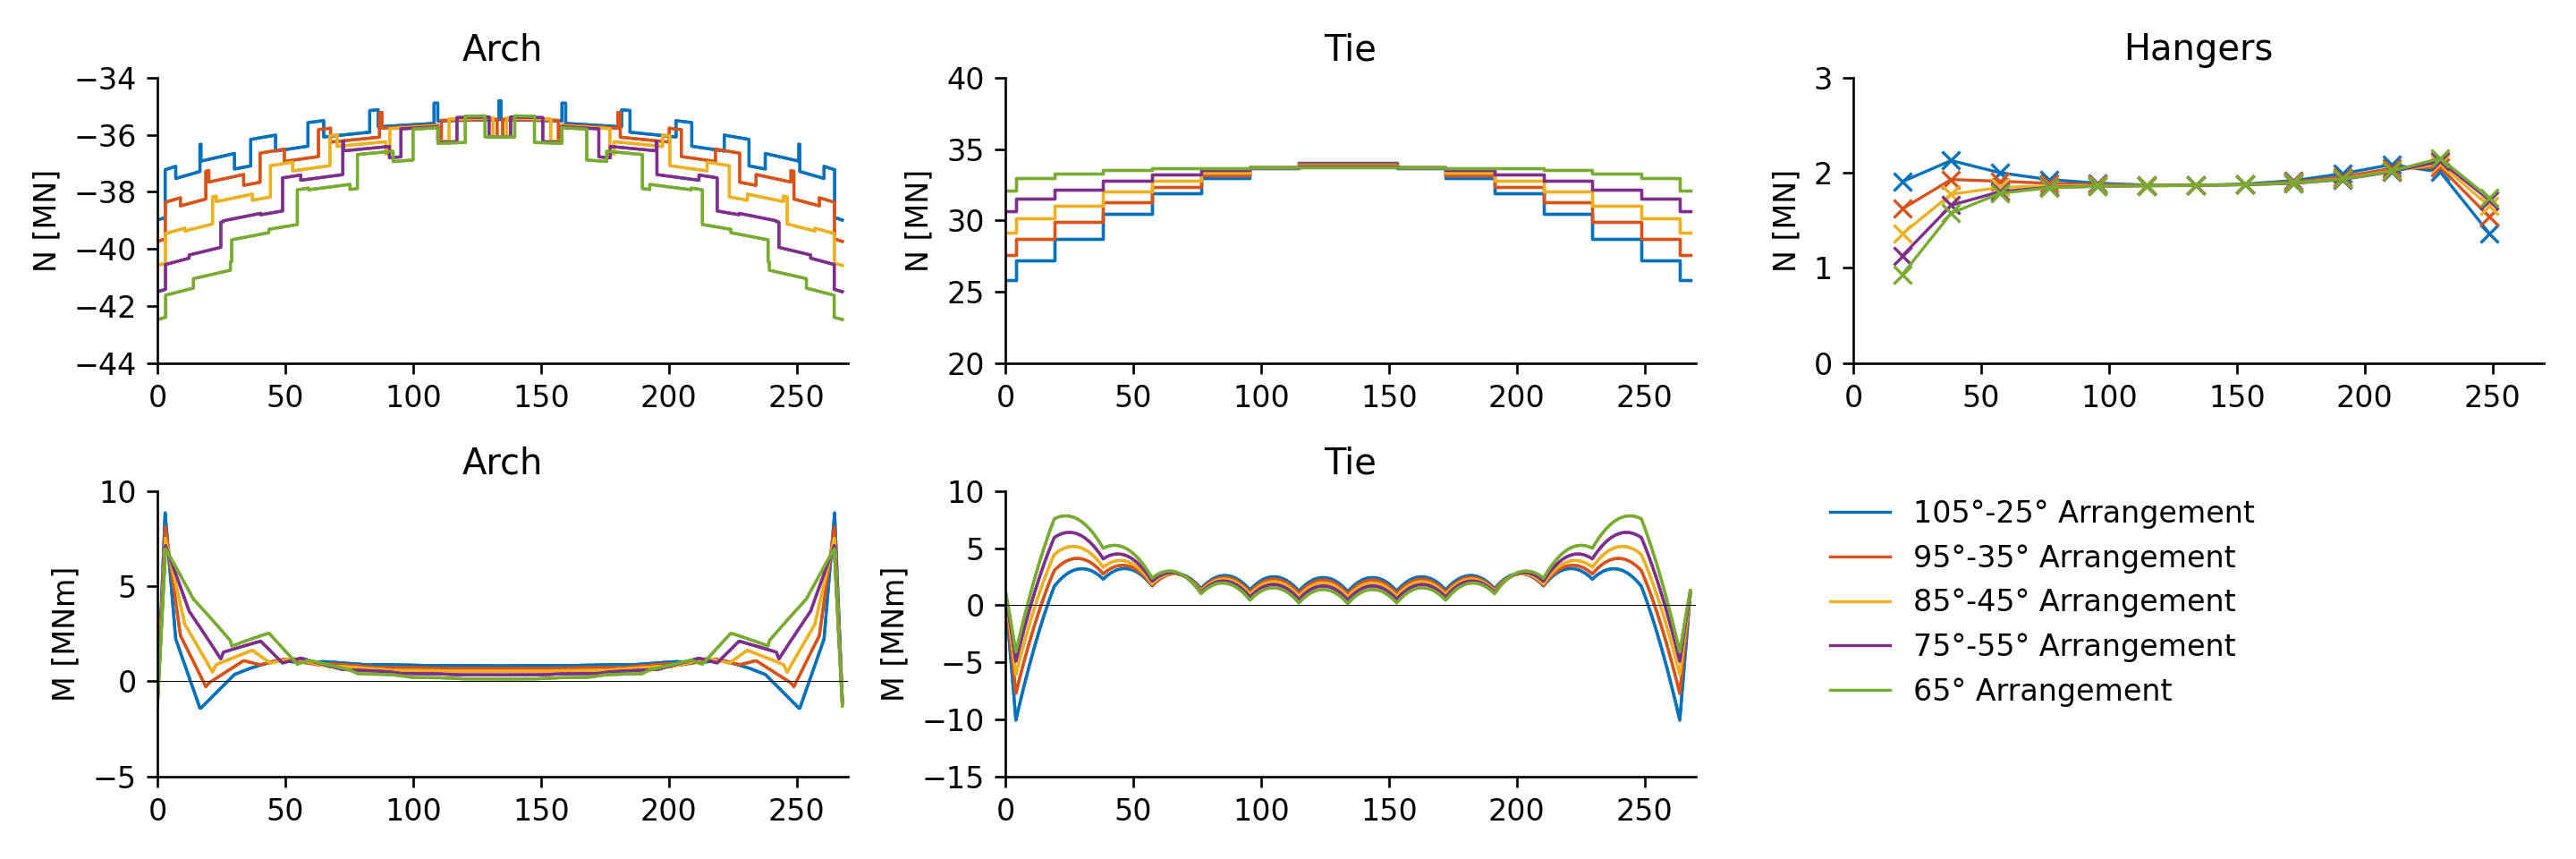
\includegraphics[trim={0 0 0 0},clip, width=\textwidth]{calculations/constant change arrangement/dead load.png}
    \caption{Elastic effects under live loading for the constant change of inclination arrangements}
    \label{fig:change_live}
\end{figure}

The parallel arrangement with a constant inclination of $65\degree$ is characterised by a significant change in the arch's normal force increasing from \SI{36}{MN} in the crown to \SI{42}{MN} at the knuckle. Further, the tie girder's normal distribution is uniform due to the mostly constant hanger forces in the span. Except near the knuckle the hangers are not efficiently used as they do not provide a strong coupling of the arch and the tie. This causes the respective elements to carry the loads on bending moments. The arrangement with a large change in inclination, on the other hand, features almost uniform hanger forces under dead loads. The moment distribution in the knuckle area is therefore minimised. A further benefit of the strong inclination changes is the relatively uniform normal force in the arch rib. It is due to the flat hangers which carry the loads toward the knuckle area resulting in an approximately radial loading and a large inclination of the thrust line at the knuckle. Also the normal force in the tie is reduced due to this effect.
Between the two extreme arrangements, the internal force effects are almost linearly distributed. For a further comparison, the range of effects under live loading is presented in \cref{}

\begin{figure}[H]
    \centering
    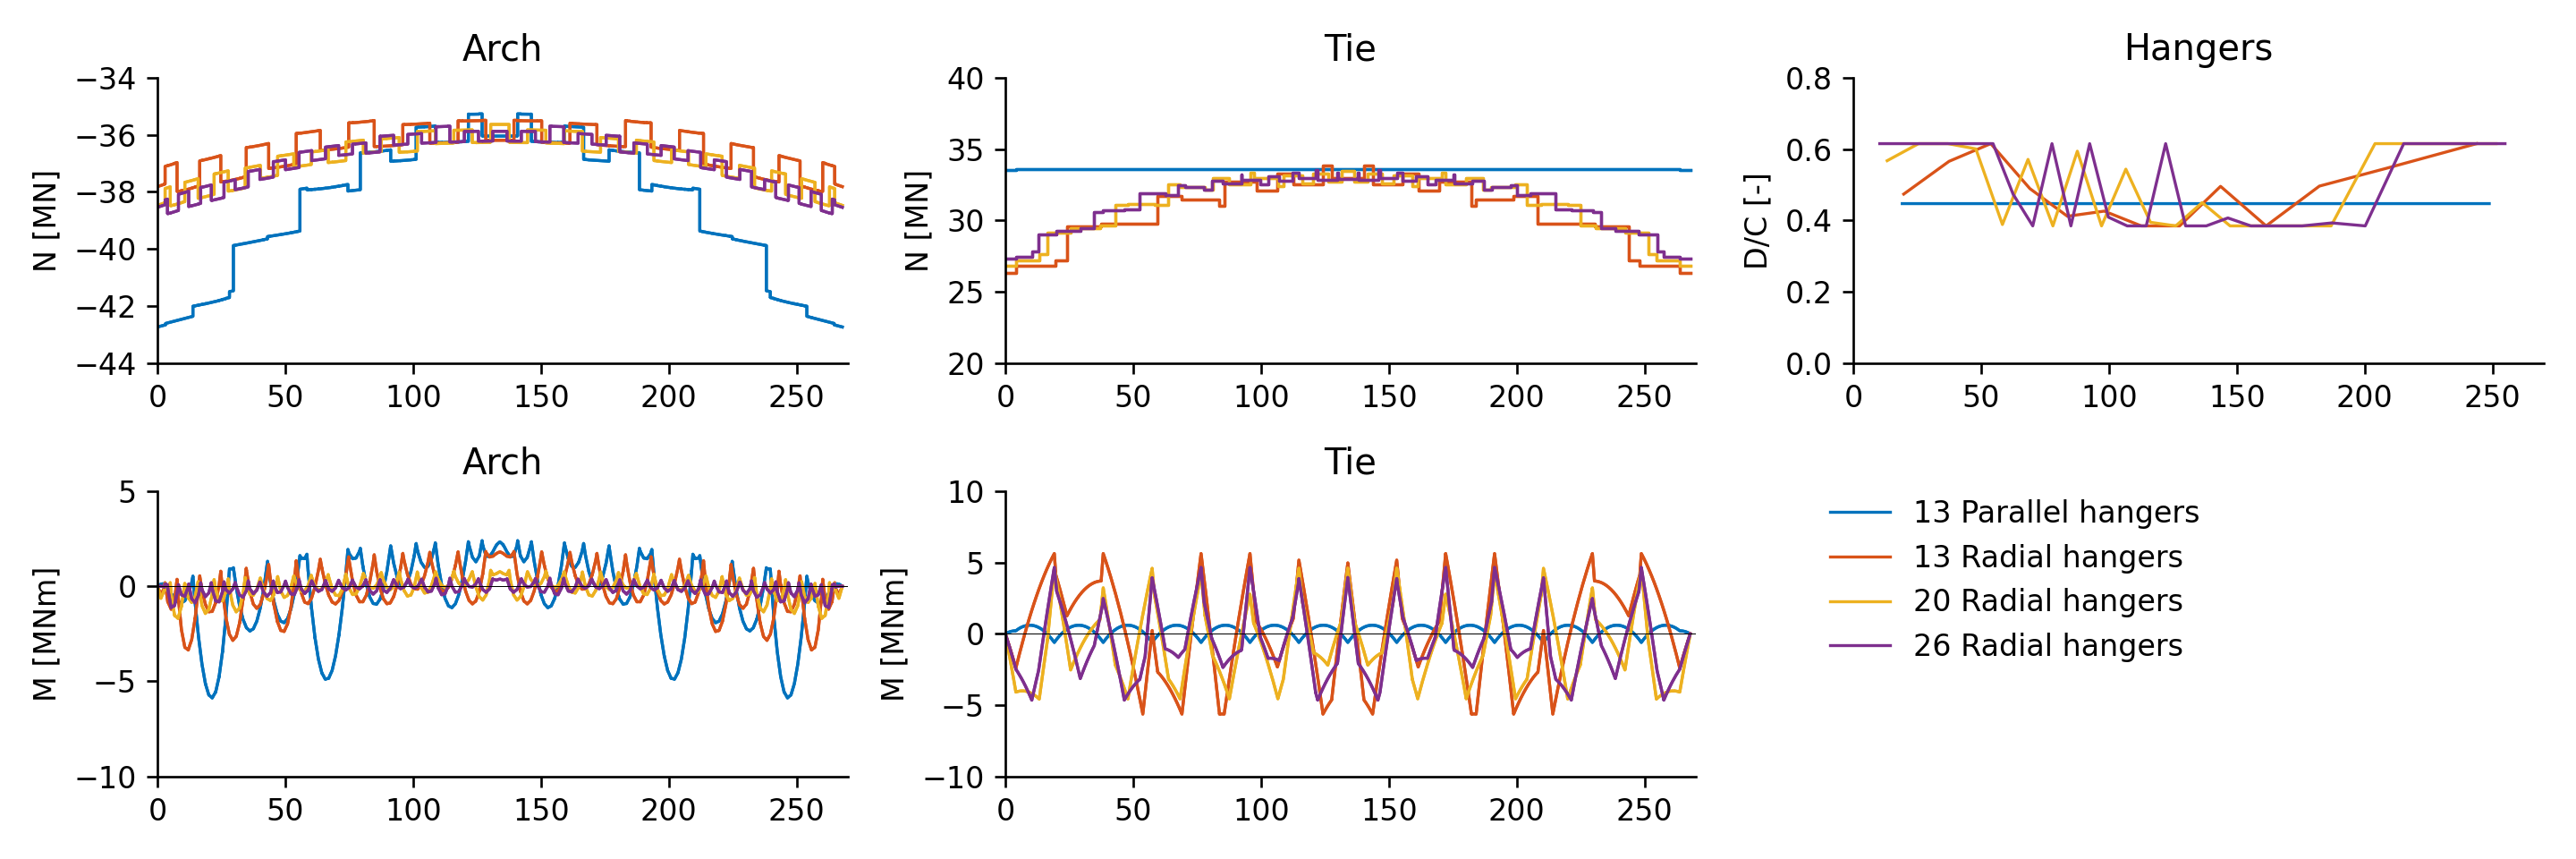
\includegraphics[trim={0 0 0 0},clip, width=0.75\textwidth]{calculations/hanger density radial/permanent.png}
    \caption{Optimised permanent effects for different hanger densities}
    \label{fig:hd_permanent_radial}
\end{figure}

\subsection{Unpatterned arrangement} \label{sec:unpatterned}



\section{Summary} \label{sec:res_summary}











